% REMEMBER: You must not plagiarise anything in your report. Be extremely careful.

\documentclass[british]{l4proj}

%
% put any additional packages here
%
\usepackage{csquotes}

\usepackage{isodate}
\usepackage{inconsolata}
\usepackage{bbm}

\usepackage{jfdm-plt}
\usepackage{mylang}
\usepackage{url}
\usepackage{cleveref}

\begin{document}

%==============================================================================
%% METADATA
\title{A Cryptographically Secure Departmental Resource Server}
\author{Christopher Watson}
\date{March 7, 2019}

\maketitle

%==============================================================================
%% ABSTRACT
\begin{abstract}
    Sharing resources securely across organisations or departments is a difficult and daunting task. Common methods rely on forms of Role-based access control (RBAC), however these cannot provide a fine-grained system for precise or modular access.\\
    This problem can be solved with the use of Attribute-based access control (ABAC) instead. Wherein, users are granted specific attributes instead of roles, allowing for any user to be given a precise and even unique set of attributes.
    Use of an Attribute-based encryption (ABE) system further improves security by handling the secure storage and transmission of resources through advanced encryption. Like ABAC, the ABE system utilises policies of attributes for users to determine if a resource should be decrypted by a given user.
    \vskip 0.5em
    This project aims to develop a full resource server product that meets the definition of "cryptographically secure". The product would be built from 2 servers: an online 'dumb' resource server to store the ABE encrypted resources and an offline 'cold storage' master key server.
    An end user would also have a locally running web client 'server' for communication with the resource server, allowing for downloading \& decryption of files, along with encryption \& uploading of their own files.
    \vskip 0.5em
    ``XYZ is bad. This project investigated ABC to determine if it was better.
    ABC used XXX and YYY to implement ZZZ. This is particularly interesting as XXX and YYY have
    never been used together. It was found that
    ABC was 20\% better than XYZ, though it caused rabies in half of subjects.''
\end{abstract}


%==============================================================================

% EDUCATION REUSE CONSENT FORM
% If you consent to your project being shown to future students for educational purposes
% then insert your name and the date below to  sign the education use form that appears in the front of the document.
% You must explicitly give consent if you wish to do so.
% If you sign, your project may be included in the Hall of Fame if it scores particularly highly.
%
% Please note that you are under no obligation to sign
% this declaration, but doing so would help future students.
%
\def\consentname {Christopher Watson} % your full name
\def\consentdate {31 January 2019} % the date you agree
%
\educationalconsent


%==============================================================================
\tableofcontents

%==============================================================================
%% Notes on formatting
%==============================================================================
% The first page, abstract and table of contents are numbered using Roman numerals and are not
% included in the page count.
%
% From now on pages are numbered
% using Arabic numerals. Therefore, immediately after the first call to \chapter we need the call
% \pagenumbering{arabic} and this should be called once only in the document.
%
% The first Chapter should then be on page 1. You are allowed 40 pages for a 40 credit project and 20 pages for a
% 20 credit report. This includes everything numbered in Arabic numerals (excluding front matter) up
% to but excluding the appendices and bibliography.
%
% You must not alter text size (it is currently 10pt) or alter margins or spacing.
%
%
%==================================================================================================================================
%
% IMPORTANT
% The chapter headings here are **suggestions**. You don't have to follow this model if
% it doesn't fit your project. Every project should have an introduction and conclusion,
% however.
%
%==================================================================================================================================
\chapter{Introduction}

% reset page numbering. Don't remove this!
\pagenumbering{arabic}

%==============================================================================
%% INTRODUCTION

Sharing resources securely across organisations or departments is a difficult task, with common methods relying on forms of \acrfull{rbac} \citep{Sandhu1996} to grant access to, often unencrypted, resource buckets. In practice, organisational hierarchies are complex in layout and depth \citep{Dooley2002}, requiring an equivalent complexity in resulting access control models. Methods such as \acrshort{rbac} are unable to provide the necessary fine-grained system for either precise or modular access, and further cannot protect the resources should the system become compromised.
\vskip 0.5em
A level of granularity is required to configure appropriate access restrictions to resources and provide long-term support for the system through dynamic access control. \acrshort{rbac} is also complex to configure properly and due to the nature of roles, can risk accidental access grants through roles that are too expansive in permissions.
\vskip 0.5em
These problems can be solved with the use of an \acrfull{abe} system, as described by \citet{Sahai2005} \& \citet{Waters2011}. Which improves security by processing the advanced encryption of resources through a proprietary policy language which allows for unique, granular access to resources on a per-user basis.

Unlike \acrshort{rbac}, an \acrshort{abe} system utilises this policy language to create bespoke, per-resource attribute policies that define specific access restrictions for the resource they are embedded into. This means that a user can only decrypt a resource if they can cryptographically prove assignment of the required attributes in their private keys \textemdash\ generated \& signed by a central \acrfull{mks}.

\section{Overview}
\label{sec:intro_overview}

This project has developed a complete resource server system, named further as the \theResServer system, which refers to the entire suite of tools developed for the system. The \theResServer system is considered complete as it encompasses all the software required to offer the secure upload \& download of shared resources to and between a set of users. Further the \theResServer system offers granular access to resources for configurable subsets of the userbase and even individuals.
\vskip 0.5em
The \theResServer system meets the definition of ``cryptographically secure''; where resources are encrypted at rest and only transmitted \& stored in a secure ciphertext format. Thus, the system would never be aware of the contents of the resources stored and implicitly, the resources will remain secure even in the event of the system becoming compromised. The product as a whole was determined to need two servers:
\begin{enumerate}
  \item an offline \emph{cold storage} \acrfull{mks} to generate user keys
  \item an online \emph{dumb} \acrfull{prs} to store and manage the \acrshort{abe} encrypted resources
\end{enumerate}

Due to the use of \acrshort{abe}, communication with the \acrshort{prs} is too complex and verbose for a standard user and so, a tool is provided for users that simplifies interactions. A user can then choose to run a simple local web client for this communication with the server, providing functionality for the download \& decryption of encrypted resources, the encryption \& upload of plaintext resources, the searching of uploaded resources and finally the management of policies \& keys for the user.

All these services are then accessible through a basic \acrshort{gui} that aims to obscure the complexity of \acrshort{abe} from the user; reducing the learning curve to use of the product.


\section{Aims}
\label{sec:intro_aims}

The main aim of the project was to produce an end product that can serve as a cryptographically secure resource server for a department and its users, with a configurable and dynamic system for access control.\\
Production of the service required careful research and design before implementation to determine both the end users of the service and the needs of the department. To achieve this, the project aimed to identify the users in the scenario of the Department of Computing Science (DCS) with an analysis of the structure of staff and students.
\vskip 0.5em
The project needed to consider the on-boarding process of bringing new users into the system and create a valid procedure for creating cryptographic keys for users. This includes determining the validity of a user's attributes and identifying an authority that can securely be tasked with performing said validation.\\
The service would have to implement and show the security of an ABE system with real-world use cases to prove its effectiveness in the scope of securely distributing resources amongst members of a department. Further, the system would also have to undergo a risk assessment to determine the actual security of the system whilst identifying risk factors within the service.
\vskip 0.5em
Since the project would implement an ABE system and it was determined that creating an ABE library was beyond the defined scope, the project also had to identify and then employ an external ABE library. Determination of which would focus on the extensibility of the library as well as evidence of the library in use for a similar scenario as a departmental resource server.\\
The project looked into the Johns Hopkins Hospital deployment of an electronic medical records system, \citet{Akinyele2011}. This represented a good scenario for comparison, as the secure distribution of medical records amongst staff and patients relied on dynamic and extremely granular access control but with an even higher requirement for security than that of a departmental resource server.
\vskip 0.5em
For the most part, the setup used for the Johns Hopkins deployment would have translated well to the project's deployment scenario, including the on-boarding process by which a user receives their private key from a central admin service and the granularity of the policies used to encrypt records.\\
However, the Johns Hopkins team required the use of mobile applications as end devices and also a need to update the user's private key remotely. Both features that were determined to be very high risk and ultimately unnecessary for the scope of the resource server. Additionally, the Johns Hopkins deployment relied on all new data coming from one source \textemdash\ the hospital \textemdash\ and so was built on the basis that one system would be able to encrypt all records. Aresource server however, must be able to receive resources from many different sources and in the project's case, any member of the DCS would need to be able to encrypt \& decrypt resources locally.


\section{Contributions}

\subsection{Policy Language}

The project produced a formal language definition of a policy language for the ABE system. This language allows the ABE system to enforce strict static typing across all policies, ensuring reliable and consistent use over all resources.\\
The formal definition includes the syntax and types for the language along with the typing rules that are enforced on a policy before encryption of a resource can be processed. The definition also includes substitution rules and the required big step semantics for the language, with a final interpretation definition to intepret the policy language to the Python bindings used in the product.

\subsection{Software}

Production of the resource service required the defining of two servers (as described above) and the creation of the services running on each. Additionally, a third product was created in order to ease use of the service for users in the form of a local web GUI client that handles communication with the resource service for the user.
\vskip 0.5em
The first server was defined as an offline master key server and would be tasked with initiating the ABE system and provisioning the master private key for the entire service. This server would remain offline from the point of complete installation, ensuring that the key is provisioned after the server enters the offline state and protecting the master private key from external internet threats.\\
The second server was defined as an online, 'dumb' storage service for the encrypted resources, only ever storing the ciphertext binary blobs with no way to decrypt or read the uploaded resources. This storage service would also be responsible for distributing the master public key, which would be manually uploaded from the master key server using some form of offline method.\\
The third product was designed to be ran locally on a user's device and then connect to the storage service in order to provide the services on offer through a simple GUI. The user provides this local client with their private user key and the service uses it to \textit{locally} decrypt resources, ensuring the key never leaves the user's device. For encrypting, the local client retrieves the master public key from the resource server and performs encryption on any required resources using the public key and the relevant policies, as defined by the user.


\section{Outline}
\label{sec:intro_outline}

\begin{enumerate}
  \item \textbf{Background}
  \begin{enumerate}
    \item Access control \& encryption
		\item Public key infrastructure \& resource servers
		\item \OpenABE library and \PyOpenABE bindings
  \end{enumerate}
  \item \textbf{Analysis/Requirements}
  \begin{enumerate}
    \item Security considerations
    \item Deployment requirements
    \item Requirements for enrolling
		\item Case Studies for deployment scenario
  \end{enumerate}
	\item \textbf{Design}
  \begin{enumerate}
    \item Design of the \thePolicyLang language
    \item Signing \& using user keys
    \item Deployment scenario \& system architecture
		\item Building policies \& searching across filenames
  \end{enumerate}
	\item \textbf{Implementation}
  \begin{enumerate}
    \item Working with the \OpenABE toolset
    \item Choosing Python's Flask for web servers
    \item Client server security
		\item Storing data with mongoDB
		\item Fuzzy string matching for filenames
  \end{enumerate}
	\item \textbf{Evaluation}
  \begin{enumerate}
    \item Security evaluation \& risk assessment
    \item Successfully achieved
    \item Failed to achieve
  \end{enumerate}
	\item \textbf{Conclusion}
  \begin{enumerate}
    \item Summary of project
    \item Future work
    \item Problems tackled during project
		\item Real-world deployment
  \end{enumerate}
\end{enumerate}


%==================================================================================================================================
\chapter{Background}
What did other people do, and how is it relevant to what you want to do?
\section{Guidance}
\begin{itemize}
    \item
      Don't give a laundry list of references.
    \item
      Tie everything you say to your problem.
    \item
      Present an argument.
    \item Think critically; weigh up the contribution of the background and put it in context.
    \item
      \textbf{Don't write a tutorial}; provide background and cite
      references for further information.
\end{itemize}

%==================================================================================================================================
\chapter{Analysis/Requirements}
What is the problem that you want to solve, and how did you arrive at it?
\section{Guidance}
Make it clear how you derived the constrained form of your problem via a clear and logical process.

%==================================================================================================================================
\chapter{Design}

\section{Requirements}
\label{sec:design_reqs}

\subsection{Deployment}

The resource server product was designed around the specific deployment scenario of the Department of Computing Science (DCS) and as such, aims to meet the requirements of users belonging to the DCS. Identified by an analysis of the DCS structure, considering students, teaching staff, technical staff \& admin staff and identifying both key roles and individuals within the organisation (see \ref{appendix:roles_users}).\\
Subsequently, the resource server focuses on the secure distribution of resources between members of a department with particular emphasis on the sharing of course resources between members of staff and the students taking their course(s).
\vskip 0.5em
This scenario also lends itself well to proving the the extensibility of the product as students have varying and changing attributes that are assigned in their private user keys - the dynamic nature of which allows the product to maintain a high level of portability.\\
This granularity in attributes, and thus policies, also provides long-term support for the product by allowing it to adapt to future changes in user structure and policy requirements.\\
Further, allowing the system to be deployed to completely new environments as the attributes can be unique to an industry and do not require definition prior to deployment.
\vskip 0.5em
The product was thus determined to require one central master key server, tasked with maintaining the master private key, provisioning the corresponding master public key and using said private key to sign new user keys.\\
A second server would handle the distribution of the master public key, storage of the encrypted resources and serving \& receiving encrypted resources.\\
Further, it was determined that for the DCS deployment, the master key server would serve as an offline or 'cold' server with no internet connection; as this provides a strong level of base security against external threats. Such offline status is possible because the master key server is not required to distribute data automatically, but rather the master public key can be manually uploaded to the resource server.

\subsection{ABE System}

As described earlier, an ABE system requires a defined policy language in order to build policies for resources to be encrypted with. This policy language describes the syntax and types of policies and is tailored to the deployment above by allowing for attributes that are required for students and staff of the DCS.\\
The ABE system required an ABE library for implementation, however since creating such a library was beyond the scope of the project, the \href{https://github.com/zeutro/openabe}{OpenABE library} from Zeutro LLC was selected instead. OpenABE was selected based upon the open source philosophy it adopts and the demonstration of its deployment as an electronic medical record system \cite{Akinyele2011}. A system that aligns well with that of a secure, departmental resource server but with even greater requirements for security.

\subsection{Resources}

Since uploaded resources have to be securely encrypted with ABE before transmission, the resource server is unaware of the contents of all resources and is in the disadvantaged position of being unable to help users identify which resources are which.\\
As such, the server must utilise a different method for resource identification and instead relies on an internal database to store metadata of resources as provided when a user performs an upload. This metadata includes filename, extension, file size and author, but most importantly keeps a record of the resource's policy in order to determine if a user should even be able to download the resource.\\
Importantly, any user \textit{could} download \textit{any} encrypted resource without risk of unauthorised decryption, however the user experience would be


\section{Formal Language Definition}
\label{sec:formal_lang}

We offer the following formal language definition for the resource server's Attribute-Based Encryption policy language, \thePolicyLang. The language was designed around the Case Studies described in \cref{sec:analysis_case_studies} and follows an extensible design principle that aims to provide a complete policy solution for the Department of Computing Science.\\
\thePolicyLang directly provides the tools for policies to be constructed for the \cref{sec:analysis_case_studies} Case Studies, which can then be interpreted to the policy format that the PyOpenABE python bindings (described in \cref{sec:bkgr_openabe}) require.
\vskip 0.5em
\thePolicyLang offers boolean comparisons for integer, string \& date attributes with further support for lists of multiple values. Additional comparison operations are provided for integer and date comparisons with `greater than', `less than' and `equivalent to' all supported, whereas booleans, strings and lists support `equivalent to' operations only.\\
This allows for integer comparisons such as ``\textit{studentLevel(\textbf{s}) $\geq$ 4}'' (as found in Case Study \#2, \cref{fig:case_study_policy_2}) and date comparisons such as ``\textit{classRepFrom(\textbf{s}) $\geq$ 17 Sep 2019}'' (as found in Case Study \#5, \cref{fig:case_study_policy_5}). String equivalence operations allow for comparisons such as ``\textit{jobField(\textbf{s}) $\equiv$ `Research \& Teaching'}'' (as found in Case Study \#1, \cref{fig:case_study_policy_1}).\\
List equivalence operations are also supported, allowing for comparisons such as ``\textit{enrolledCourses(\textbf{s}) $\equiv$ [1001, 1017]}'' (as found in Case Study \#2 \cref{fig:case_study_policy_2}) where the policy requires both that `\textit{enrolledCourses(\textbf{s})}' resolves to a list and that that list contains the elements in `\textit{[1001, 1017]}'.

\section{Abstract Syntax, Types, \& Contexts}\label{sec:defs}

\begin{figure}[ht]
  \centering
\begin{align*}
  \ty{n}{\mathbb{Z}}
  &
    \Coloneqq
    \text{Integers}
  & \text{Values}
  \\
  \ty{b}{\mathbb{B}}
  & \Coloneqq
    \mathsf{False}\alt\mathsf{True}
  \\
  \ty{d}{\mathbb{D}}
  & \Coloneqq
    \text{Dates}
  \\
  \ty{s}{\mathbb{S}}
  & \Coloneqq
    \text{Strings}
  \\
  v
  &
    \Coloneqq
    n
    \alt
    b
    \alt
    d
    \alt
    s
  \\
  \ty{l}{\mathbb{L}_T}
  & \Coloneqq
    \emptyset_T\alt{}v\Cons_T{}l
  \\
  e
  &
    \Coloneqq
    v
    \alt
    l
  & \text{Expressions}
  \\
  &
    \firstAlt
    \exprEQ{e}{e}
    \alt
    \exprGT{e}{e}
    \alt
    \exprLT{e}{e}
  \\
  & \firstAlt
    \exprGTE{e}{e}
    \alt
    \exprLTE{e}{e}
  &
  \\
  & \firstAlt
    \exprOr{e}{e}
    \alt
    \exprAnd{e}{e}
  &
  \\
  &
    \firstAlt
    \left( \lambda \mu \bullet e \right)
    \alt
    e \; \$ \; e
  &
    \text{Statements}
  \\
  T
  &
    \Coloneqq
    \mathbb{Z}
    \alt
    \mathbb{B}
    \alt
    \mathbb{D}
    \alt
    \mathbb{S}
    \alt
    \mathbb{L}
    \alt
    {T \rightarrow{} T}
  &
    \text{Types}
  \\
  \Gamma
  &
    \Coloneqq
    \envAdd{(\ty{x}{T})}
    \alt
    \emptyset
    &
      \text{Context}
\end{align*}
  \caption{\label{fig:syntax}The policy language's abstract syntax, types, and context.}
\end{figure}

\Cref{fig:syntax} presents the syntactical structure, and types for our language.
Our language contains Integers, Boolean, Date, String and List values, we leave abstract how integers and dates are written.

Integers \& Dates can be compared using standard comparison operations of: \texttt{greater-than}, \texttt{less-than} and \texttt{equals-to}, as well as \texttt{greater-than-or-equal-to} and \texttt{less-than-or-equal-to}.
Boolean operators provide logical conjunction and disjunction.

A context ($\Gamma$) keeps track of well-typed expressions, and our context can be expanded.


\subsection{Typing Rules}
\label{subsec:typing-rules}

\begin{figure}[ht]
  \centering
\begin{mathpar}
  \infer*[left=Intro-Int]
  {
    \\
  }
  {
    \ty{i}{\TyInt}
  }
  \and
  \infer*[left=Intro-Bool]
  {
    \\
  }
  {
    \ty{b}{\mathbb{B}}
  }
  \and
  \infer*[left=Intro-Date]
  {
    \\
  }
  {
    \ty{d}{\mathbb{D}}
  }
  \and
  \infer*[left=Intro-String]
  {
    \\
  }
  {
    \ty{s}{\mathbb{S}}
  }
  \and
  \infer*[left=Intro-Empty]
  {
    \env{\ty{a}{T}}\\
    \left[ T \in T_l \right]
  }
  {
    \env{\ty{\emptyset_a}{\mathbb{L}_a}}
  }
  \and
  \infer*[left=Intro-Cons]
  {
    \env{\ty{v}{a}}\\
    \env{\ty{l}{\mathbb{L}_a}}\\
    \env{\ty{a}{T}}\\
    \left[ T \in T_l \right]
  }
  {
    \env{\ty{v\Cons_t{}l}{\mathbb{L}_a}}
  }
  \and
  \infer*[left=OR]
  {
    \env{\ty{a}{\mathbb{B}}}\\
    \env{\ty{b}{\mathbb{B}}}
  }
  {
    \env{\ty{\exprOr{a}{b}}{\mathbb{B}}}
  }
  \and
  \infer*[left=AND]
  {
    \env{\ty{a}{\mathbb{B}}}\\
    \env{\ty{b}{\mathbb{B}}}
  }
  {
    \env{\ty{\exprAnd{a}{b}}{\mathbb{B}}}
  }
  \and
  \infer*[left=GT]
  {
    \env{\ty{a}{T}}\\
    \env{\ty{b}{T}}\\
    \left[ T \in \{ \mathbb{Z}, \mathbb{D} \} \right]
  }
  {
    \env{\ty{\exprGT{a}{b}}{\mathbb{B}}}
  }
  \and
  \infer*[left=LT]
  {
    \env{\ty{a}{T}}\\
    \env{\ty{b}{T}}\\
    \left[ T \in \{ \mathbb{Z}, \mathbb{D} \} \right]
  }
  {
    \env{\ty{\exprLT{a}{b}}{\mathbb{B}}}
  }
  \and
  \infer*[left=EQ]
  {
    \env{\ty{a}{T}}\\
    \env{\ty{b}{T}}\\
    \left[ T \in \{ \mathbb{Z}, \mathbb{B}, \mathbb{D}, \mathbb{S}, \mathbb{L}_t \} \right]
  }
  {
    \env{\ty{\exprEQ{a}{b}}{\mathbb{B}}}
  }
  \and
  \infer*[left=GTE]
  {
    \env{\ty{a}{T}}\\
    \env{\ty{b}{T}}\\
    \left[ T \in \{ \mathbb{Z}, \mathbb{D} \} \right]
  }
  {
    \env{\ty{\exprGTE{a}{b}}{\mathbb{B}}}
  }
  \and
  \infer*[left=LTE]
  {
    \env{\ty{a}{T}}\\
    \env{\ty{b}{T}}\\
    \left[ T \in \{ \mathbb{Z}, \mathbb{D} \} \right]
  }
  {
    \env{\ty{\exprLTE{a}{b}}{\mathbb{B}}}
  }
\end{mathpar}
  \caption{\label{fig:rules}The formal definition of the Typing Rules for \thePolicyLang}
\end{figure}

\Cref{fig:rules} presents the \thePolicyLang typing rules.
These rules dictate what it means for an expression/statement to be well-formed within \thePolicyLang and for any expression/statement in \thePolicyLang, we use the typing rules to construct a derivation that provides proof that the expression/statement is well-typed, that is we can apply each rule and form a derivation tree. If we cannot construct this tree then the expression is ill-typed and syntactically not valid.

The Typing Rules define 5 base cases for the 5 value types \thePolicyLang supports (as defined in \cref{fig:syntax}), meaning instances of the 5 types derive directly to their type. Next, the boolean logical operators OR \& AND are defined as requiring two Boolean parameters that also derive to a Boolean type return. The standard comparison operators \textbf{$>$}, \textbf{$<$}, \textbf{$>=$} \& \textbf{$<=$} all take two parameters of a matching type, where the type may be Integer or Date, and derives to a Boolean response. Lastly, the \textbf{$==$} comparison similarly takes two parameters of a matching type, but where the type may be Integer, Boolean, Date, String or List, and also derives to a Boolean return.


\subsection{Substitution}
\label{subsec:substitution}

\begin{figure}[ht]
  \centering
\begin{align*}
  \subst{\mu}{e}{x}
  &
    \Coloneqq
    \begin{cases}
      e&x\equiv\mu\\
      x&x\not\equiv\mu\\
    \end{cases}
  \\
  \subst{\exprOr{a}{b}}{e}{x}&\Coloneqq\exprOr{\subst{a}{e}{x}}{\subst{b}{e}{x}}\\
  \subst{\exprAnd{a}{b}}{e}{x}&\Coloneqq\exprAnd{\subst{a}{e}{x}}{\subst{b}{e}{x}}\\
  \subst{\exprGT{a}{b}}{e}{x}&\Coloneqq\exprGT{\subst{a}{e}{x}}{\subst{b}{e}{x}}\\
  \subst{\exprLT{a}{b}}{e}{x}&\Coloneqq\exprLT{\subst{a}{e}{x}}{\subst{b}{e}{x}}\\
  \subst{\exprEQ{a}{b}}{e}{x}&\Coloneqq\exprEQ{\subst{a}{e}{x}}{\subst{b}{e}{x}}\\
  \subst{\exprGTE{a}{b}}{e}{x}&\Coloneqq\exprGTE{\subst{a}{e}{x}}{\subst{b}{e}{x}}\\
  \subst{\exprLTE{a}{b}}{e}{x}&\Coloneqq\exprLTE{\subst{a}{e}{x}}{\subst{b}{e}{x}}
\end{align*}
  \caption{\label{fig:subst}The formal definition of the Substitution Rules for \thePolicyLang}
\end{figure}

\Cref{fig:subst} presents a standard set of substitution rules for \thePolicyLang.
These rules describe how we can iterate over our expressions/statements in \thePolicyLang and through recursive calls, swap variables for values.\\
Starting with expressions and variables, we describe when $\mu$ is an expression or variable. Next we describe the resolving of the \textbf{or} \& \textbf{and} logical operators' parameters to expressions and variables, followed by similar descriptions for the standard comparisons \textbf{greaterThan}, \textbf{lessThan}, \textbf{equal}, \textbf{greaterThanEqual} \& \textbf{lessThanEqual}.\\
Through the recursive calls, we eventually reach a state where we have visited all expressions \& statements and we can swap in values in place of all variables by working backwards through the recursive calls.


\subsection{Big Step Semantics}
\label{subsec:semantics}

\begin{figure}[ht]
  \centering
\begin{mathpar}
  \infer*[left=$\mathbb{Z}$]
  {
    \\
  }
  {
    i\Downarrow{}\primed{i}
  }
  \and
  \infer*[left=$\mathbb{B}$]
  {
    \\
  }
  {
    b\Downarrow{}\primed{b}
  }
  \and
  \infer*[left=$\mathbb{D}$]
  {
    \\
  }
  {
    d\Downarrow{}\primed{d}
  }
  \and
  \infer*[left=$\mathbb{S}$]
  {
    \\
  }
  {
    s\Downarrow{}\primed{s}
  }
  \and
  \infer*[left=$\mathbb{L}$]
  {
    \\
  }
  {
    l\Downarrow{}\primed{l}
  }
  \and
  \infer*[left=OR]
  {
    a\Downarrow{}\primed{a}\\
    b\Downarrow{}\primed{b}
  }
  {
    \exprOr{a}{b}\Downarrow\primed{a}\vee\primed{b}
  }
  \and
  \infer*[left=AND]
  {
    a\Downarrow{}\primed{a}\\
    b\Downarrow{}\primed{b}
  }
  {
    \exprAnd{a}{b}\Downarrow\primed{a}\wedge\primed{b}
  }
  \and
  \infer*[left=GT]
  {
    a\Downarrow{}\primed{a}\\
    b\Downarrow{}\primed{b}
  }
  {
    \exprGT{a}{b}\Downarrow\primed{a}>\primed{b}
  }
  \and
  \infer*[left=LT]
  {
    a\Downarrow{}\primed{a}\\
    b\Downarrow{}\primed{b}
  }
  {
    \exprLT{a}{b}\Downarrow\primed{a}<\primed{b}
  }
  \and
  \infer*[left=EQ]
  {
    a\Downarrow{}\primed{a}\\
    b\Downarrow{}\primed{b}
  }
  {
    \exprEQ{a}{b}\Downarrow\primed{a}\equiv\primed{b}
  }
  \and
  \infer*[left=GTE]
  {
    a\Downarrow{}\primed{a}\\
    b\Downarrow{}\primed{b}
  }
  {
    \exprGTE{a}{b}\Downarrow\primed{a}\geq\primed{b}
  }
  \and
  \infer*[left=LTE]
  {
    a\Downarrow{}\primed{a}\\
    b\Downarrow{}\primed{b}
  }
  {
    \exprLTE{a}{b}\Downarrow\primed{a}\leq\primed{b}
  }
  \end{mathpar}
  \caption{\label{fig:semantics}The formal definition of the Big Step Semantics for \thePolicyLang}
\end{figure}

\Cref{fig:semantics} presents the Big-Step semantics for \thePolicyLang, here we use \emph{real} operations to show how an expression is reduced using \emph{real} integer and boolean operators.\\
Operational semantics describe how we evaluate our programs, describing how we can \emph{reduce} the \thePolicyLang language expressions and statements to a single value. Here we present the Big-Step semantics of evaluating expressions to describe the transition from an expression to the final result, skipping over the intermediate computations (as described in \citet{Myers2007}).\\
This intentionally abstracts away the finer details of the operations required to evaluate an individual expression, but still presents the syntactic process. This abstraction was considered beneficial since the expressions available in \thePolicyLang are frequently used across many languages and other resources are available that better describe the Small Step semantics of similar expressions (see \citet{Sewell2009, DBLP:conf/lomaps/Schmidt96}).


\subsection{Interpretation}
\label{subsec:interpretation}

\begin{figure}[ht]
  \centering
\begin{align*}
  \textsc{\thePolicyLang}&\rightarrow\textsc{Python (PyOpenABE)}\\
  \interpB{\TyInt}&\Coloneqq\text{\ttfamily int}\\
  \interpB{\mathbb{B}}&\Coloneqq\text{\ttfamily bool}\\
  \interpB{\mathbb{D}}&\Coloneqq\text{\ttfamily datetime.date}\\
  \interpB{\mathbb{S}}&\Coloneqq\text{\ttfamily str}\\
  \interpB{\mathbb{L}}&\Coloneqq\text{\ttfamily list}\\
  \interpB{n}&\Coloneqq\text{\ttfamily int(}n\text{\ttfamily)}\\
  \interpB{\EnumFalse}&\Coloneqq\text{\ttfamily False}\\
  \interpB{\EnumTrue} &\Coloneqq\text{\ttfamily True}\\
  \interpB{d}&\Coloneqq\text{\ttfamily datetime.date(}d\text{\ttfamily)}\\
  \interpB{s}&\Coloneqq\text{\ttfamily str(}s\text{\ttfamily)}\\
  \interpB{l_s}&\Coloneqq\text{\ttfamily [}\interpB{l}\alt l \leftarrow l_s\text{\ttfamily]}\\
  \interpB{sub}&\Coloneqq\interpB{sub}_{s}\\
  \interpB{proj_{sub}}&\Coloneqq\interpB{proj_{sub}}_{s}\\
  \interpB{env}&\Coloneqq\interpB{env}_{e}\\
  \interpB{proj_{env}}&\Coloneqq\interpB{proj_{env}}_{e}\\
  \interpB{res}&\Coloneqq\interpB{res}_{r}\\
  \interpB{proj_{res}}&\Coloneqq\interpB{proj_{res}}_{r}\\
  \interpB{\exprOr{a}{b}}  &\Coloneqq\interpB{a}\,\text{\ttfamily or}\,\interpB{b}\\
  \interpB{\exprAnd{a}{b}} &\Coloneqq\interpB{a}\,\text{\ttfamily and}\,\interpB{b}\\
  \interpB{\exprGT{a}{b}}  &\Coloneqq\interpB{a}\,\text{\ttfamily \textgreater}\,\interpB{b}\\
  \interpB{\exprLT{a}{b}}  &\Coloneqq\interpB{a}\,\text{\ttfamily \textless}\,\interpB{b}\\
  \interpB{\exprEQ{a}{b}}  &\Coloneqq\interpB{a}\,\text{\ttfamily ==}\,\interpB{b}\\
  \interpB{\exprGTE{a}{b}}  &\Coloneqq\interpB{a}\,\text{\ttfamily \textgreater =}\,\interpB{b}\\
  \interpB{\exprLTE{a}{b}}  &\Coloneqq\interpB{a}\,\text{\ttfamily \textless =}\,\interpB{b}
\end{align*}
  \caption{\label{fig:interp}The formal definition of the Interpretation Rules for \thePolicyLang}
\end{figure}

In this final section we describe how we interpret \thePolicyLang to another form, in this case concrete Python expressions for the \PyOpenABE bindings library (described in \Cref{subsec:bkgr_pyopenabe}), with \cref{fig:interp} presenting these Interpretation rules and like substitution, interpretation recursively operates over each statement and expression in \thePolicyLang. At each step replacing the expression from \thePolicyLang with it's equivalent Python form. As we are interpreting \thePolicyLang we do not provide operational semantics, since Python provides this for us.


\section{User Key Design}
\label{sec:design_user_key}


%==================================================================================================================================
\chapter{Implementation}
What did you do to implement this idea, and what technical achievements did you make?
\section{Guidance}
You can't talk about everything. Cover the high level first, then cover important, relevant or impressive details.



\section{General points}

These points apply to the whole dissertation, not just this chapter.



\subsection{Figures}
\emph{Always} refer to figures included, like Figure \ref{fig:relu}, in the body of the text. Include full, explanatory captions and make sure the figures look good on the page.
You may include multiple figures in one float, as in Figure \ref{fig:synthetic}, using \texttt{subcaption}, which is enabled in the template.



% Figures are important. Use them well.
\begin{figure}
    \centering
    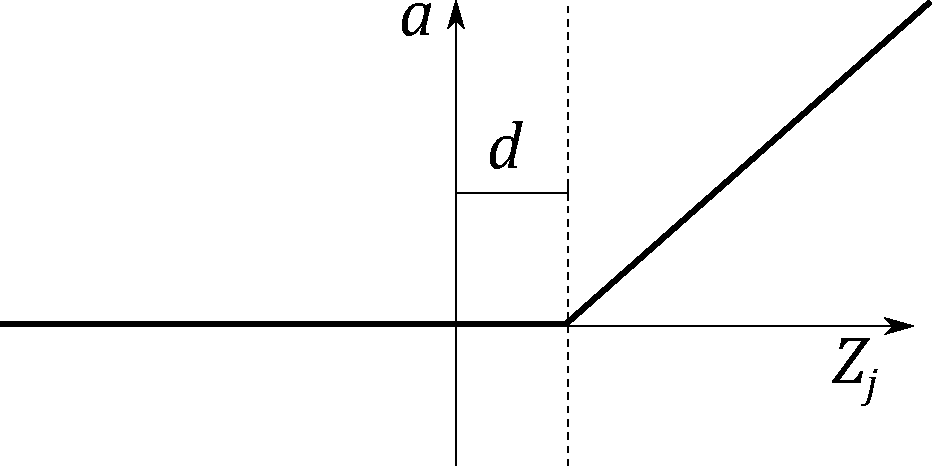
\includegraphics[width=0.5\linewidth]{images/relu.pdf}

    \caption{In figure captions, explain what the reader is looking at: ``A schematic of the rectifying linear unit, where $a$ is the output amplitude,
    $d$ is a configurable dead-zone, and $Z_j$ is the input signal'', as well as why the reader is looking at this:
    ``It is notable that there is no activation \emph{at all} below 0, which explains our initial results.''
    \textbf{Use vector image formats (.pdf) where possible}. Size figures appropriately, and do not make them over-large or too small to read.
    }

    % use the notation fig:name to cross reference a figure
    \label{fig:relu}
\end{figure}


\begin{figure}
    \centering
    \begin{subfigure}[b]{0.45\textwidth}
        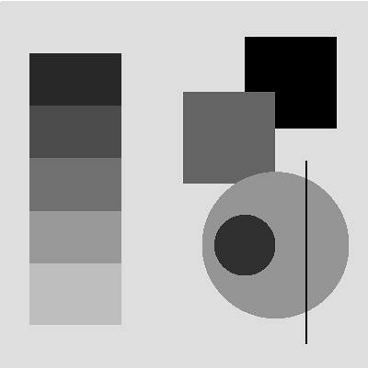
\includegraphics[width=\textwidth]{images/synthetic.png}
        \caption{Synthetic image, black on white.}
        \label{fig:syn1}
    \end{subfigure}
    ~ %add desired spacing between images, e. g. ~, \quad, \qquad, \hfill etc.
      %(or a blank line to force the subfigure onto a new line)
    \begin{subfigure}[b]{0.45\textwidth}
        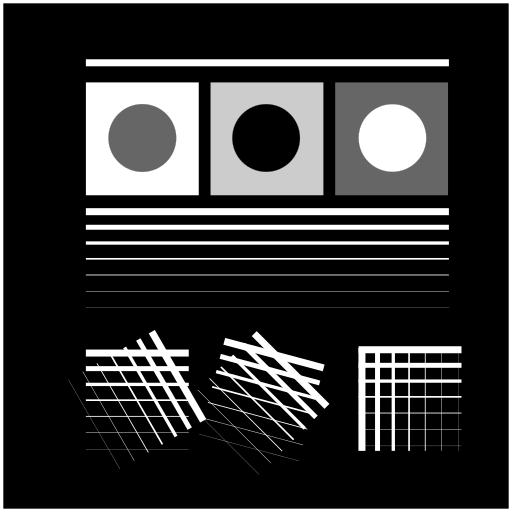
\includegraphics[width=\textwidth]{images/synthetic_2.png}
        \caption{Synthetic image, white on black.}
        \label{fig:syn2}
    \end{subfigure}
    ~ %add desired spacing between images, e. g. ~, \quad, \qquad, \hfill etc.
    %(or a blank line to force the subfigure onto a new line)
    \caption{Synthetic test images for edge detection algorithms. \subref{fig:syn1} shows various gray levels that require an adaptive algorithm. \subref{fig:syn2}
    shows more challenging edge detection tests that have crossing lines. Fusing these into full segments typically requires algorithms like the Hough transform.
    This is an example of using subfigures, with \texttt{subref}s in the caption.
    }\label{fig:synthetic}
\end{figure}

\clearpage

\subsection{Equations}

Equations should be typeset correctly and precisely. Make sure you get parenthesis sizing correct, and punctuate equations correctly
(the comma is important and goes \textit{inside} the equation block). Explain any symbols used clearly if not defined earlier.

For example, we might define:
\begin{equation}
    \hat{f}(\xi) = \frac{1}{2}\left[ \int_{-\infty}^{\infty} f(x) e^{2\pi i x \xi} \right],
\end{equation}
where $\hat{f}(\xi)$ is the Fourier transform of the time domain signal $f(x)$.

\subsection{Algorithms}
Algorithms can be set using \texttt{algorithm2e}, as in Algorithm \ref{alg:metropolis}.

% NOTE: line ends are denoted by \; in algorithm2e
\begin{algorithm}
    \DontPrintSemicolon
    \KwData{$f_X(x)$, a probability density function returing the density at $x$.\; $\sigma$ a standard deviation specifying the spread of the proposal distribution.\;
    $x_0$, an initial starting condition.}
    \KwResult{$s=[x_1, x_2, \dots, x_n]$, $n$ samples approximately drawn from a distribution with PDF $f_X(x)$.}
    \Begin{
        $s \longleftarrow []$\;
        $p \longleftarrow f_X(x)$\;
        $i \longleftarrow 0$\;
        \While{$i < n$}
        {
            $x^\prime \longleftarrow \mathcal{N}(x, \sigma^2)$\;
            $p^\prime \longleftarrow f_X(x^\prime)$\;
            $a \longleftarrow \frac{p^\prime}{p}$\;
            $r \longleftarrow U(0,1)$\;
            \If{$r<a$}
            {
                $x \longleftarrow x^\prime$\;
                $p \longleftarrow f_X(x)$\;
                $i \longleftarrow i+1$\;
                append $x$ to $s$\;
            }
        }
    }

\caption{The Metropolis-Hastings MCMC algorithm for drawing samples from arbitrary probability distributions,
specialised for normal proposal distributions $q(x^\prime|x) = \mathcal{N}(x, \sigma^2)$. The symmetry of the normal distribution means the acceptance rule takes the simplified form.}\label{alg:metropolis}
\end{algorithm}

\subsection{Tables}

If you need to include tables, like Table \ref{tab:operators}, use a tool like https://www.tablesgenerator.com/ to generate the table as it is
extremely tedious otherwise.

\begin{table}[]
    \caption{The standard table of operators in Python, along with their functional equivalents from the \texttt{operator} package. Note that table
    captions go above the table, not below. Do not add additional rules/lines to tables. }\label{tab:operators}
    %\tt
    \rowcolors{2}{}{gray!3}
    \begin{tabular}{@{}lll@{}}
    %\toprule
    \textbf{Operation}    & \textbf{Syntax}                & \textbf{Function}                            \\ %\midrule % optional rule for header
    Addition              & \texttt{a + b}                          & \texttt{add(a, b)}                                    \\
    Concatenation         & \texttt{seq1 + seq2}                    & \texttt{concat(seq1, seq2)}                           \\
    Containment Test      & \texttt{obj in seq}                     & \texttt{contains(seq, obj)}                           \\
    Division              & \texttt{a / b}                          & \texttt{div(a, b) }  \\
    Division              & \texttt{a / b}                          & \texttt{truediv(a, b) } \\
    Division              & \texttt{a // b}                         & \texttt{floordiv(a, b)}                               \\
    Bitwise And           & \texttt{a \& b}                         & \texttt{and\_(a, b)}                                  \\
    Bitwise Exclusive Or  & \texttt{a \textasciicircum b}           & \texttt{xor(a, b)}                                    \\
    Bitwise Inversion     & \texttt{$\sim$a}                        & \texttt{invert(a)}                                    \\
    Bitwise Or            & \texttt{a | b}                          & \texttt{or\_(a, b)}                                   \\
    Exponentiation        & \texttt{a ** b}                         & \texttt{pow(a, b)}                                    \\
    Identity              & \texttt{a is b}                         & \texttt{is\_(a, b)}                                   \\
    Identity              & \texttt{a is not b}                     & \texttt{is\_not(a, b)}                                \\
    Indexed Assignment    & \texttt{obj{[}k{]} = v}                 & \texttt{setitem(obj, k, v)}                           \\
    Indexed Deletion      & \texttt{del obj{[}k{]}}                 & \texttt{delitem(obj, k)}                              \\
    Indexing              & \texttt{obj{[}k{]}}                     & \texttt{getitem(obj, k)}                              \\
    Left Shift            & \texttt{a \textless{}\textless b}       & \texttt{lshift(a, b)}                                 \\
    Modulo                & \texttt{a \% b}                         & \texttt{mod(a, b)}                                    \\
    Multiplication        & \texttt{a * b}                          & \texttt{mul(a, b)}                                    \\
    Negation (Arithmetic) & \texttt{- a}                            & \texttt{neg(a)}                                       \\
    Negation (Logical)    & \texttt{not a}                          & \texttt{not\_(a)}                                     \\
    Positive              & \texttt{+ a}                            & \texttt{pos(a)}                                       \\
    Right Shift           & \texttt{a \textgreater{}\textgreater b} & \texttt{rshift(a, b)}                                 \\
    Sequence Repetition   & \texttt{seq * i}                        & \texttt{repeat(seq, i)}                               \\
    Slice Assignment      & \texttt{seq{[}i:j{]} = values}          & \texttt{setitem(seq, slice(i, j), values)}            \\
    Slice Deletion        & \texttt{del seq{[}i:j{]}}               & \texttt{delitem(seq, slice(i, j))}                    \\
    Slicing               & \texttt{seq{[}i:j{]}}                   & \texttt{getitem(seq, slice(i, j))}                    \\
    String Formatting     & \texttt{s \% obj}                       & \texttt{mod(s, obj)}                                  \\
    Subtraction           & \texttt{a - b}                          & \texttt{sub(a, b)}                                    \\
    Truth Test            & \texttt{obj}                            & \texttt{truth(obj)}                                   \\
    Ordering              & \texttt{a \textless b}                  & \texttt{lt(a, b)}                                     \\
    Ordering              & \texttt{a \textless{}= b}               & \texttt{le(a, b)}                                     \\
    % \bottomrule
    \end{tabular}
    \end{table}
\subsection{Code}

Avoid putting large blocks of code in the report (more than a page in one block, for example). Use syntax highlighting if possible, as in Listing \ref{lst:callahan}.

\begin{lstlisting}[language=python, float, caption={The algorithm for packing the $3\times 3$ outer-totalistic binary CA successor rule into a
    $16\times 16\times 16\times 16$ 4 bit lookup table, running an equivalent, notionally 16-state $2\times 2$ CA.}, label=lst:callahan]
    def create_callahan_table(rule="b3s23"):
        """Generate the lookup table for the cells."""
        s_table = np.zeros((16, 16, 16, 16), dtype=np.uint8)
        birth, survive = parse_rule(rule)

        # generate all 16 bit strings
        for iv in range(65536):
            bv = [(iv >> z) & 1 for z in range(16)]
            a, b, c, d, e, f, g, h, i, j, k, l, m, n, o, p = bv

            # compute next state of the inner 2x2
            nw = apply_rule(f, a, b, c, e, g, i, j, k)
            ne = apply_rule(g, b, c, d, f, h, j, k, l)
            sw = apply_rule(j, e, f, g, i, k, m, n, o)
            se = apply_rule(k, f, g, h, j, l, n, o, p)

            # compute the index of this 4x4
            nw_code = a | (b << 1) | (e << 2) | (f << 3)
            ne_code = c | (d << 1) | (g << 2) | (h << 3)
            sw_code = i | (j << 1) | (m << 2) | (n << 3)
            se_code = k | (l << 1) | (o << 2) | (p << 3)

            # compute the state for the 2x2
            next_code = nw | (ne << 1) | (sw << 2) | (se << 3)

            # get the 4x4 index, and write into the table
            s_table[nw_code, ne_code, sw_code, se_code] = next_code

        return s_table

\end{lstlisting}

%==================================================================================================================================
\chapter{Evaluation}
How good is your solution? How well did you solve the general problem, and what evidence do you have to support that?

\section{Guidance}
\begin{itemize}
    \item
        Ask specific questions that address the general problem.
    \item
        Answer them with precise evidence (graphs, numbers, statistical
        analysis, qualitative analysis).
    \item
        Be fair and be scientific.
    \item
        The key thing is to show that you know how to evaluate your work, not
        that your work is the most amazing product ever.
\end{itemize}

\section{Evidence}
Make sure you present your evidence well. Use appropriate visualisations, reporting techniques and statistical analysis, as appropriate.

If you visualise, follow the basic rules, as illustrated in Figure \ref{fig:boxplot}:
\begin{itemize}
\item Label everything correctly (axis, title, units).
\item Caption thoroughly.
\item Reference in text.
\item \textbf{Include appropriate display of uncertainty (e.g. error bars, Box plot)}
\item Minimize clutter.
\end{itemize}

See the file \texttt{guide\_to\_visualising.pdf} for further information and guidance.

\begin{figure}
    \centering
    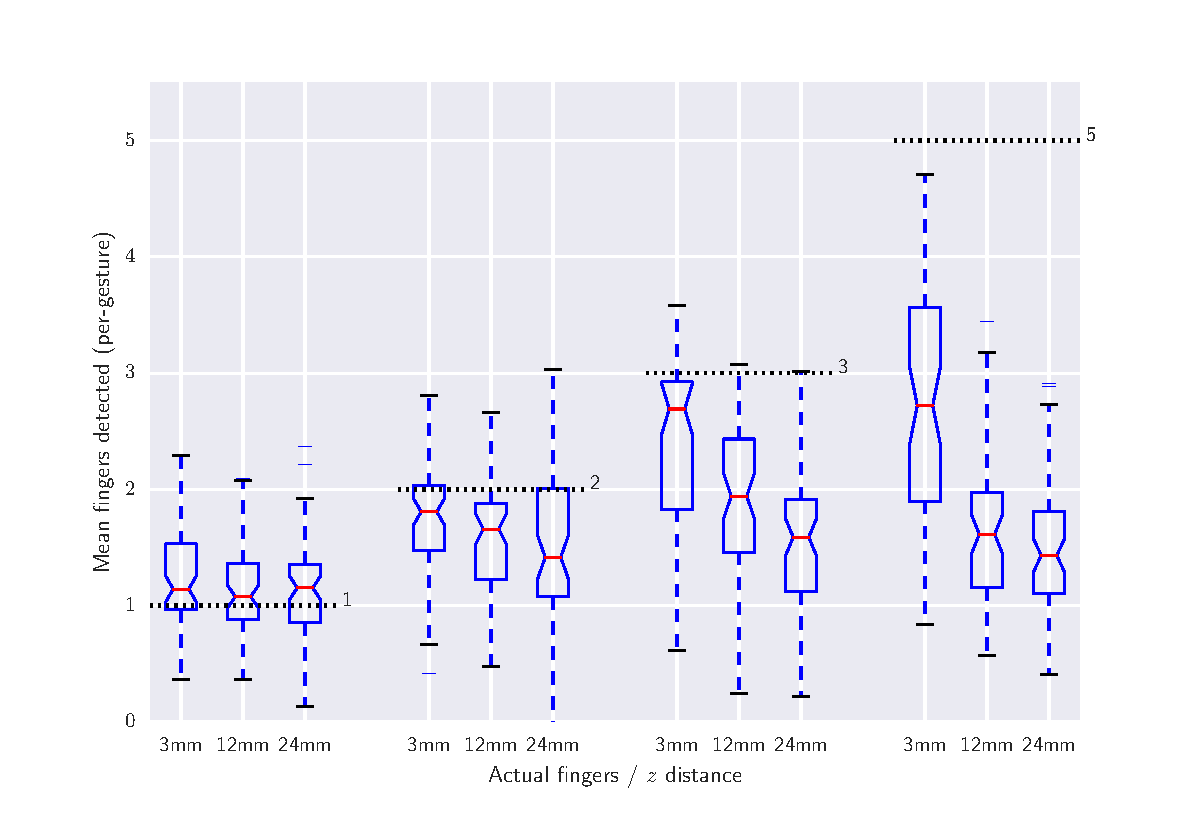
\includegraphics[width=1.0\linewidth]{images/boxplot_finger_distance.pdf}

    \caption{Average number of fingers detected by the touch sensor at different heights above the surface, averaged over all gestures. Dashed lines indicate
    the true number of fingers present. The Box plots include bootstrapped uncertainty notches for the median. It is clear that the device is biased toward
    undercounting fingers, particularly at higher $z$ distances.
    }

    % use the notation fig:name to cross reference a figure
    \label{fig:boxplot}
\end{figure}


%==================================================================================================================================
\chapter{Conclusion}
Summarise the whole project for a lazy reader who didn't read the rest (e.g. a prize-awarding committee).
\section{Guidance}
\begin{itemize}
    \item
        Summarise briefly and fairly.
    \item
        You should be addressing the general problem you introduced in the
        Introduction.
    \item
        Include summary of concrete results (``the new compiler ran 2x
        faster'')
    \item
        Indicate what future work could be done, but remember: \textbf{you
        won't get credit for things you haven't done}.
\end{itemize}

%==================================================================================================================================
%
%
%==================================================================================================================================
%  APPENDICES

\begin{appendices}

\chapter{Appendices}
\label{ch:appendices}

\section{Appendix A - Deployment Roles \& Users}
\label{appendix:roles_users}

\Cref{fig:appendix_roles_users} presents the identified user roles of the \acrfull{dcs} in red, to the left, and the identified users in blue, to the right. Also see (Electronic Appendix \ref{appendix:e_roles_users}).

\begin{figure}[htp]
    \centering
    \label{fig:appendix_roles_users}
    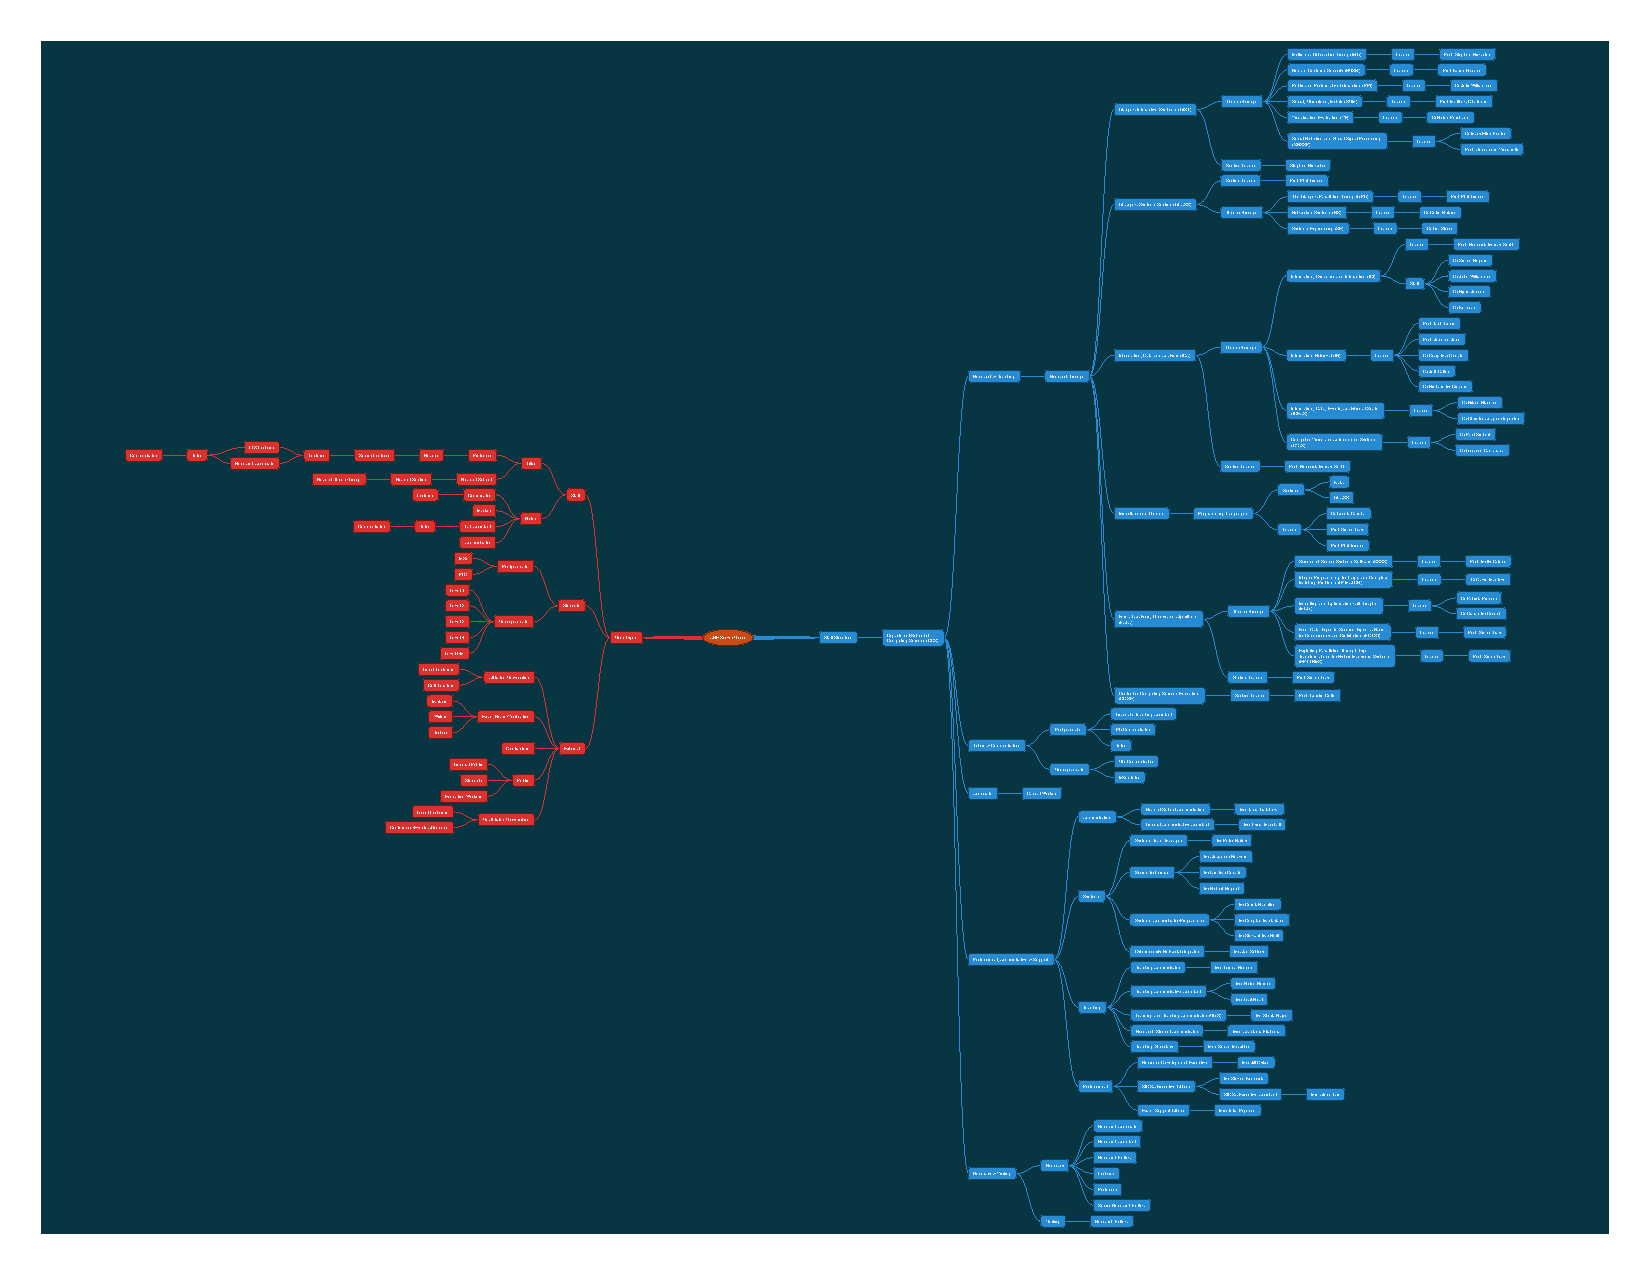
\includegraphics[width=\linewidth]{appendices/mind_maps/ABE_Users_slides_Oct26.pdf}
    \caption{Mind Map representing the different users \& roles identified for a \acrshort{dcs} deployment.}
\end{figure}

\section{Appendix B - Environment Attributes}
\label{appendix:environments}

\Cref{fig:appendix_environments} presents the identified environment attributes for the \acrfull{dcs}. Also see (Electronic Appendix \ref{appendix:e_environments}).

\begin{figure}[htp]
    \centering
    \label{fig:appendix_environments}
    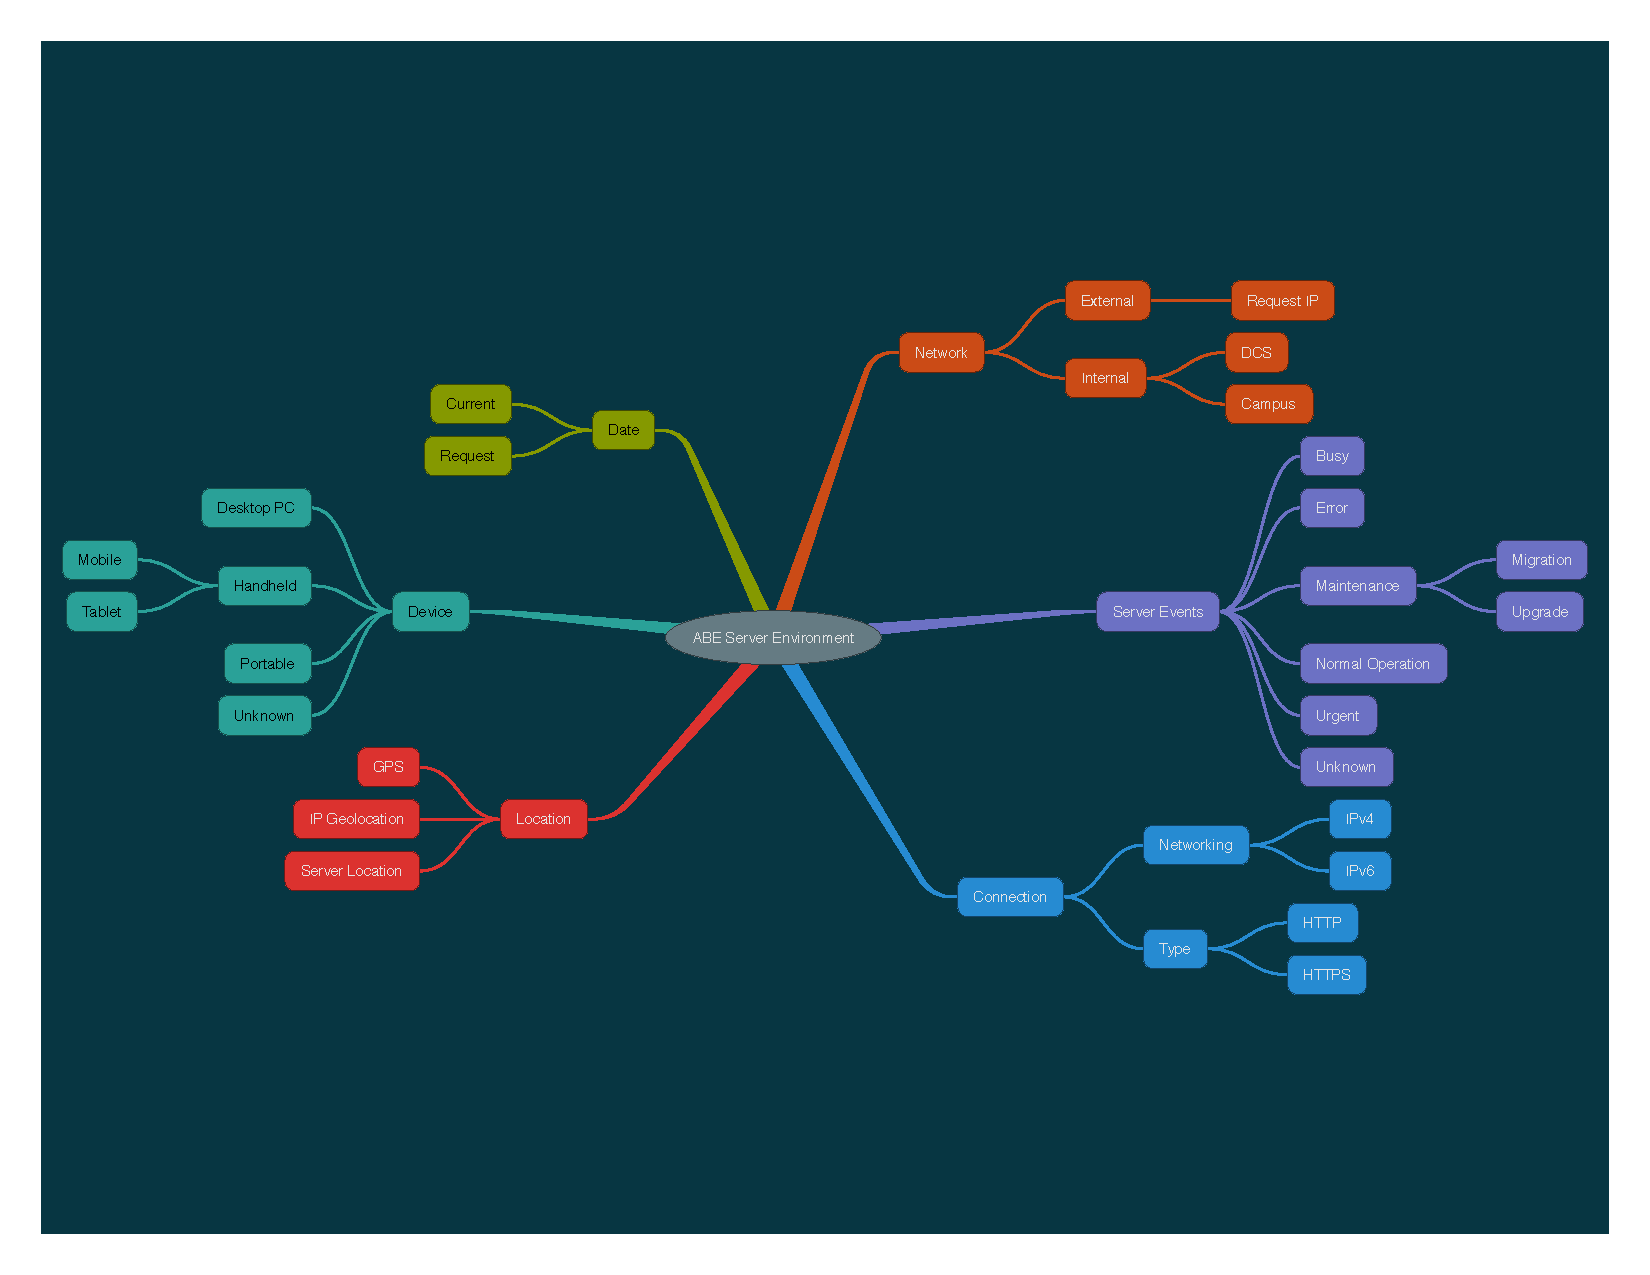
\includegraphics[width=\linewidth]{appendices/mind_maps/ABE_Environments_slides_Oct26.pdf}
    \caption{Mind Map representing the different environment attributes identified for a \acrshort{dcs} deployment.}
\end{figure}

\section{Appendix C - System Use Cases}
\label{appendix:use_cases}

\Cref{fig:appendix_use_cases} presents the identified use cases for the \acrfull{dcs}. Also see (Electronic Appendix \ref{appendix:e_use_cases}).

\begin{figure}[htp]
    \centering
    \label{fig:appendix_use_cases}
    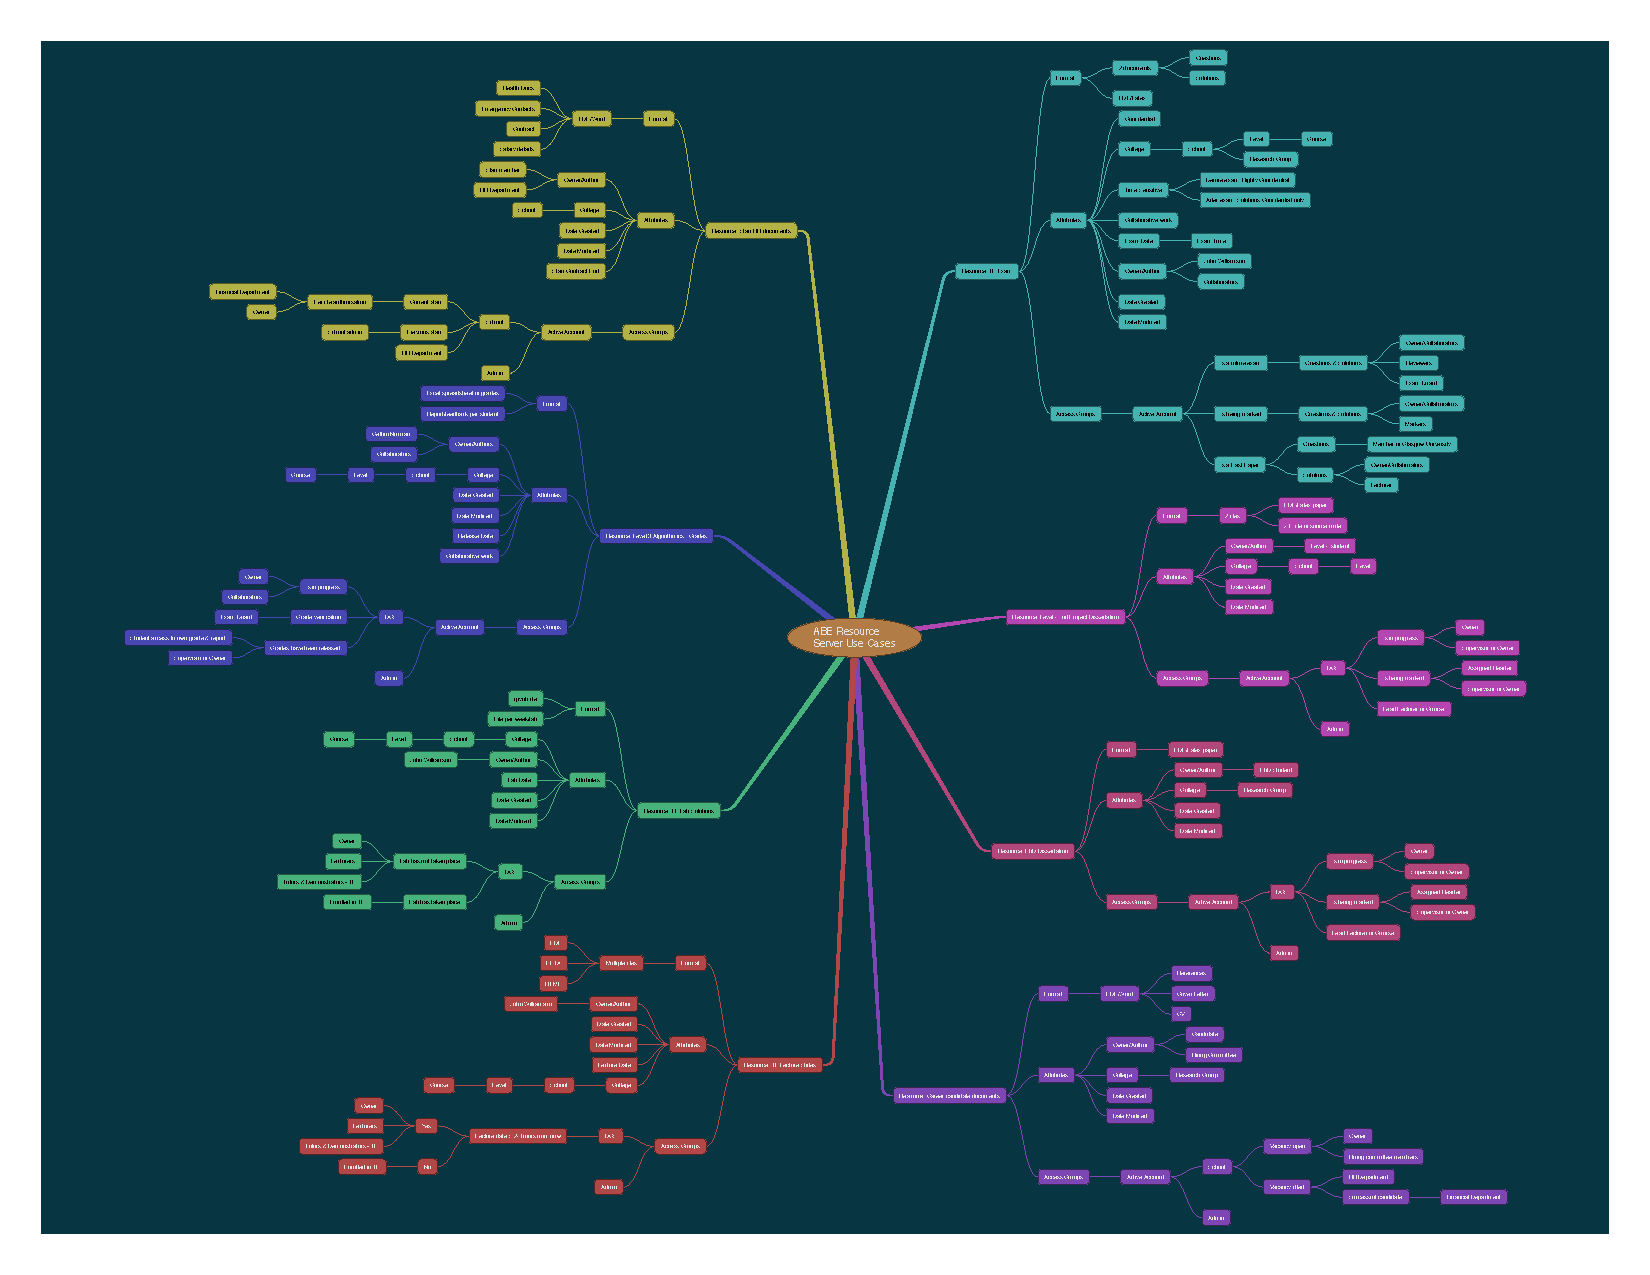
\includegraphics[width=\linewidth]{appendices/mind_maps/ABE_Use_Cases_slides_Oct26.pdf}
    \caption{Mind Map representing the different use cases identified for a \acrshort{dcs} deployment.}
\end{figure}

\section{Appendix D - Enrolment Diagram for Staff User}
\label{appendix:enrolment_diagram}

\Cref{fig:appendix_sta_deployment} represents a deployment diagram for the \theResServer system, with staff member enrolling into the system. This diagram is an alternative to the student enrolment diagram in \Cref{fig:deployment_diagram}.

The staff member can be seen requesting a user key \#1 (and providing their staff username) from the \acrshort{dcs} Teaching Assistant, whom verifies the staff members's identity and then retrieves their details \#2 from the HR/Payroll system. The Teaching Assistant then processes the returned attributes \#5 for the Master Key Server, and then requests a new key \#6 by providing the student's attributes. The Master Key Server can be seen processing \#7 and then returning the newly generated key \#8 to the Teaching Assistant, whom finally provides the key to the staff member.

\begin{figure}[htp]
    \centering
    \label{fig:appendix_sta_deployment}
    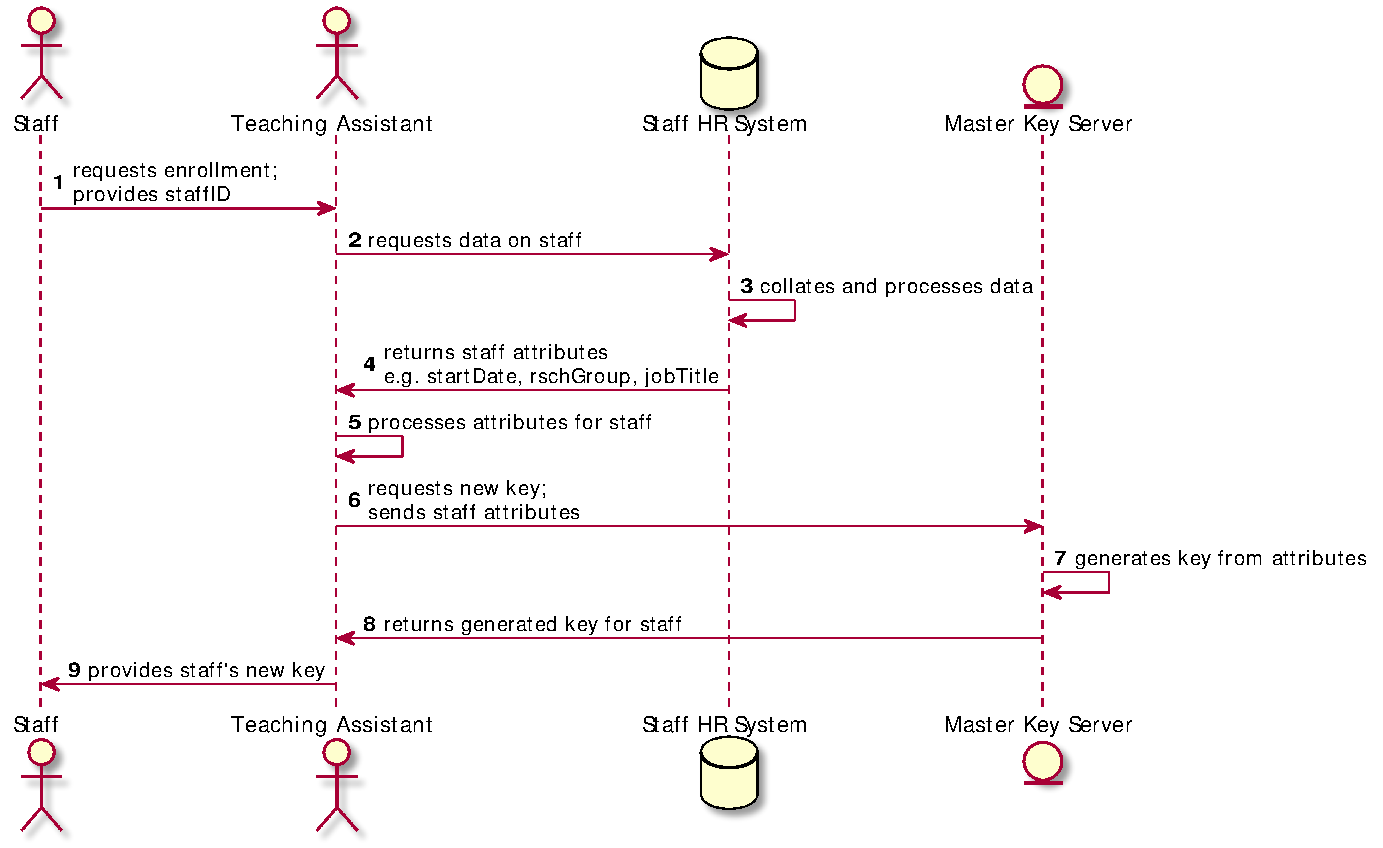
\includegraphics[width=\linewidth,keepaspectratio]{appendices/diagrams/flow_of_info/enrollment_sta_sequence.pdf}

    \caption{A sequence diagram demonstrating the enrolment process for a staff member.}

\end{figure}

\section{Appendix E - System Architecture Diagram}
\label{appendix:architecture_diagram}

\Cref{fig:appendix_sys_arch_full} represents a system architecture diagram for the \theResServer system. This diagram is an alternative to the condensed system architecture diagram in \Cref{fig:sys_arch_abbrv}.

The \acrfull{mks} is shown in an offline state with access to a local copy of the \OpenABE library for provisioning the system \& generating user keys. The \acrfull{prs} is shown receiving offline updates from the \acrshort{mks}, managing a local database with resource metadata \& the associated resource storage and providing search, config and upload \& download interfaces for clients. The \acrfull{crs} is shown with local access to an \OpenABE library for encryption \& decryption and access to an abstract Authentication Service (such as the university's SSO system). The \acrshort{crs} also implements the search, config and upload \& download interfaces provided by the \acrshort{prs} and provides its own upload \& download, encrypt \& decrypt and resource search interfaces for the user.

\begin{figure}[htp]
    \centering
    \label{fig:appendix_sys_arch_full}
    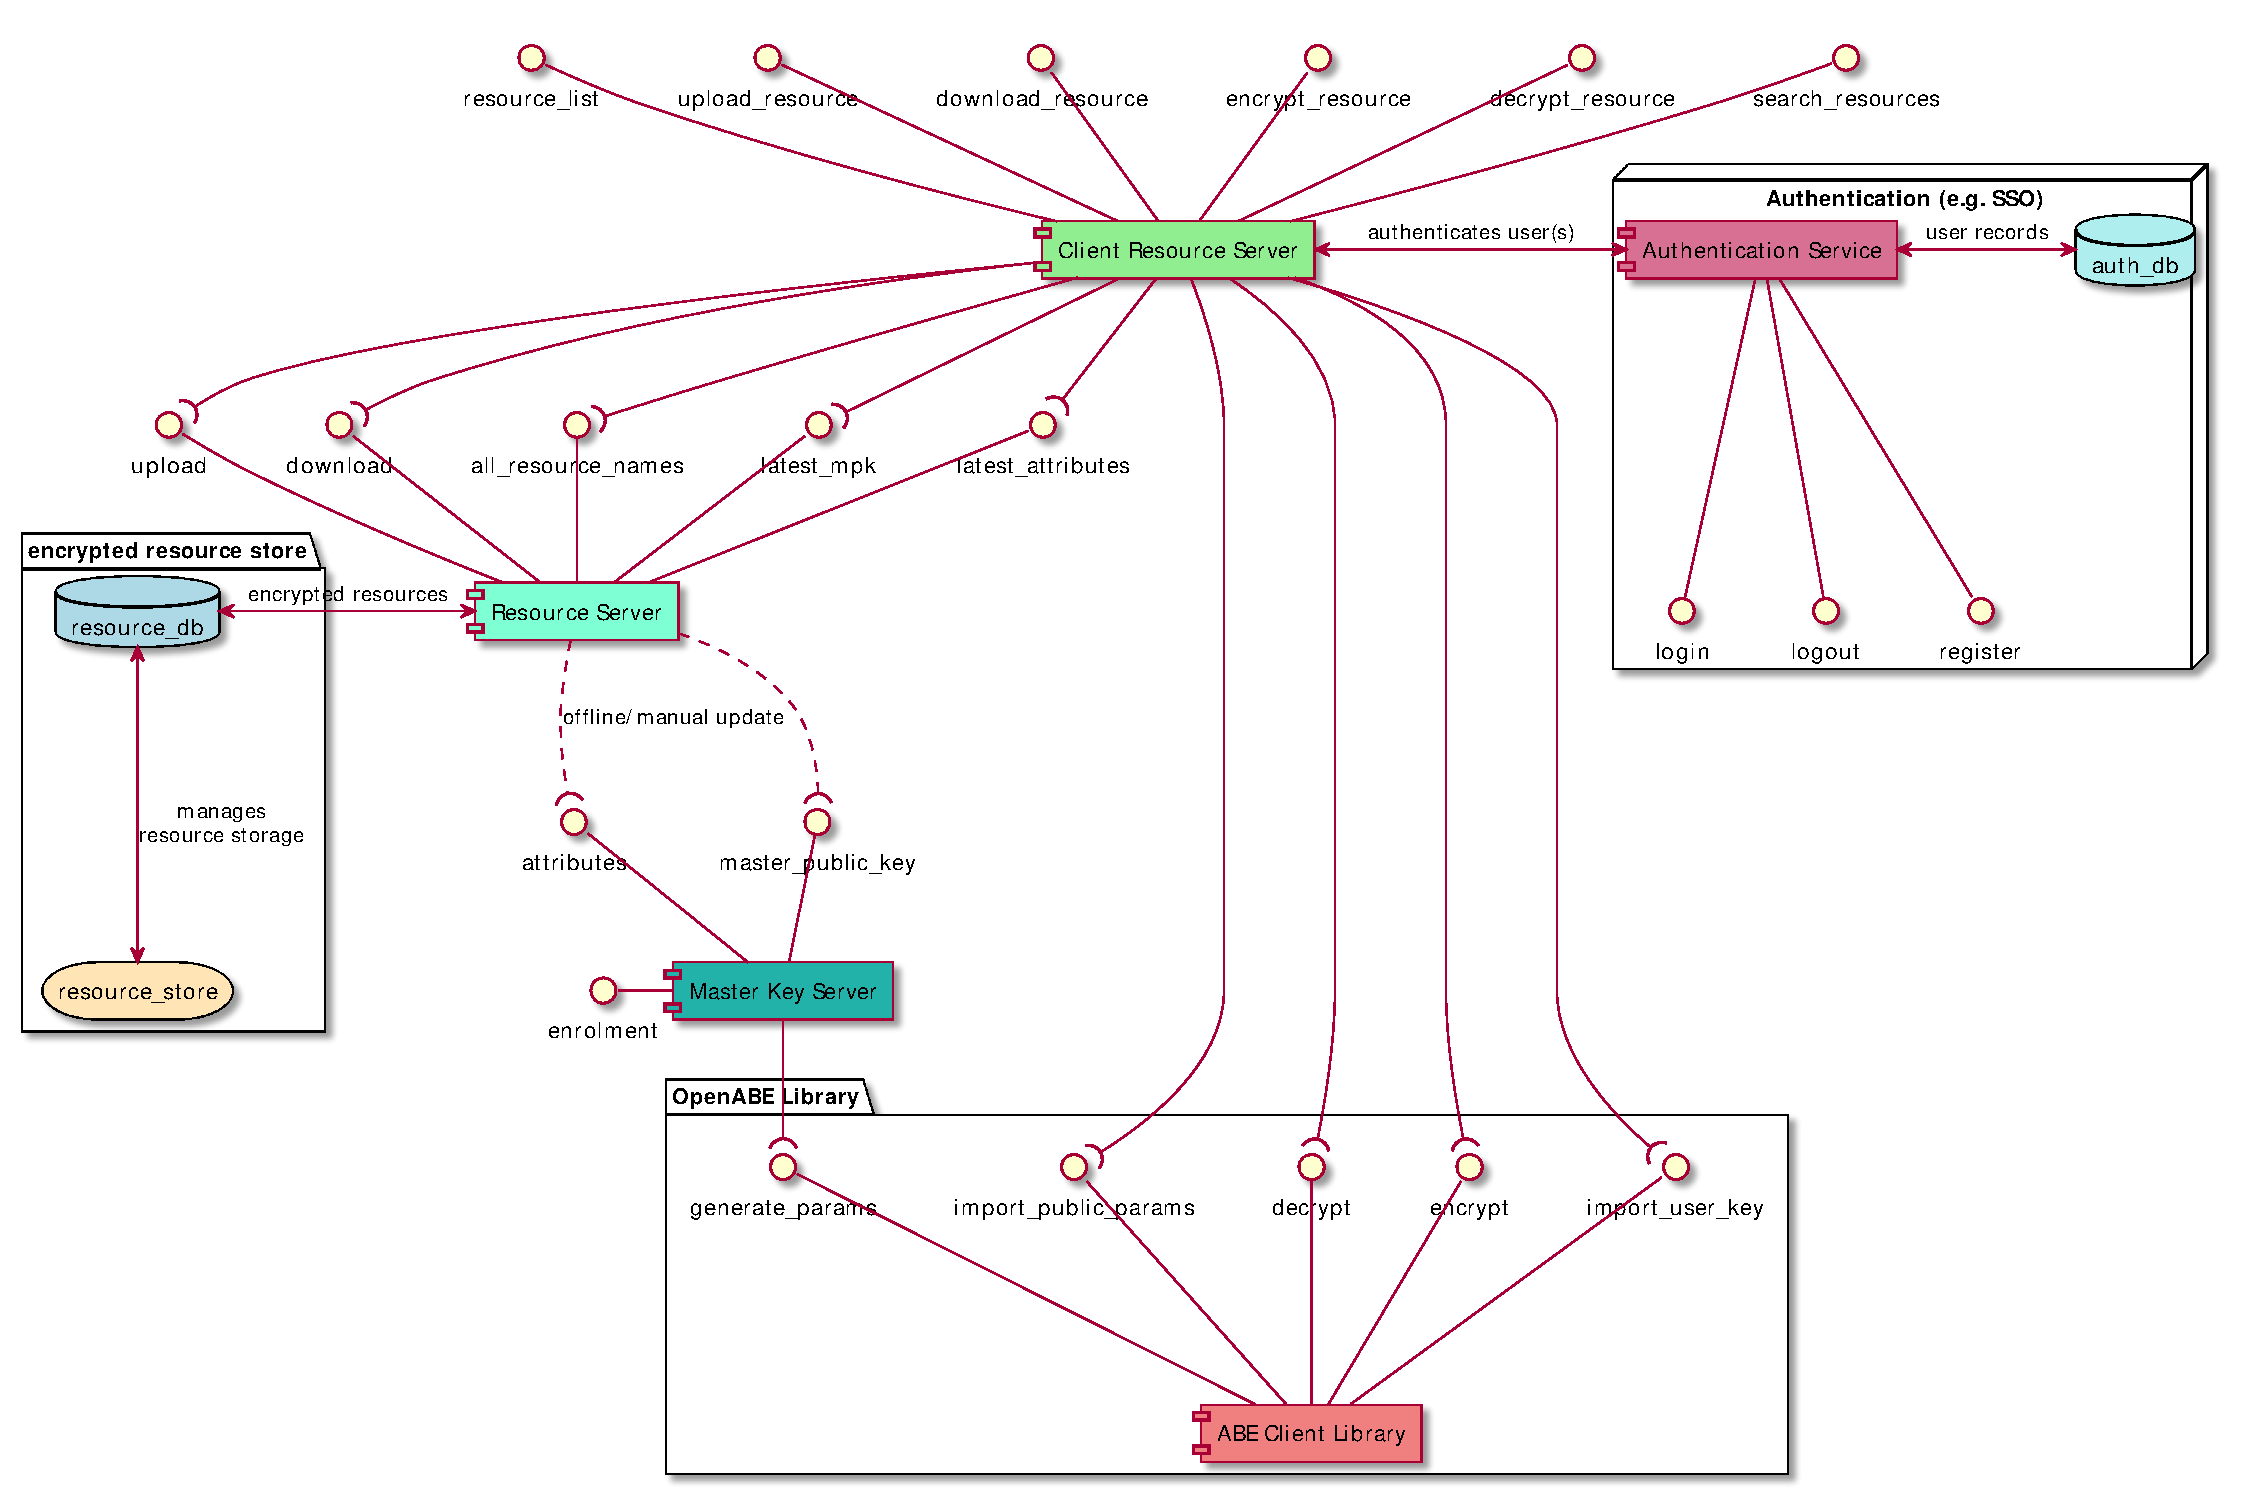
\includegraphics[width=\linewidth,keepaspectratio]{appendices/diagrams/infrastructure/system_architecture.pdf}

    \caption{
      A full architecture diagram describing the system architecture of the \theResServer system.
    }

\end{figure}

\section{Appendix F - Implementing Case Study \#0 with \thePolicyLang}
\label{appendix:case_study_0_policy}

For this study the following details have been assumed:
\begin{itemize}
  \item
    the solutions were encrypted and then uploaded by the Admin staff member
  \item
    the staff member is Teresa Bonner with username `tbonner'
\end{itemize}
\vskip 0.5em
With the details extracted, we can determine the attributes for the policy, where we define \textbf{\textit{Subject} s} and \textbf{\textit{Environment} e} as:
\begin{itemize}
  \item[]
    \textbf{s} $\Rightarrow$ role, accountActiveUntil, username
  \item[]
    \textbf{e} $\Rightarrow$ currentDate
\end{itemize}

Applying the identified attributes for Case Study \#0 (\Cref{subsec:analysis_case_studies_0}) provides the policy in \cref{fig:case_study_policy_0} which would have been embedded in the encrypted lecture slides by the staff member before upload. The encrypted past paper can then remain stored on the server but only accessible to staff members and students.

\begin{figure}[ht]
  \centering
\begin{align*}
  \text{Policy(\textbf{s},\textbf{e})}
  &
    \leftarrow
    \text{username(\textbf{s})} \equiv \text{`tbonner'}
  \\
  &
    \phantom{::}\vee
    \text{role(\textbf{s})} \equiv \text{`Staff'} \mid \text{`Student'}
  \\
  &
    \phantom{::}\wedge
    \text{accountActiveUntil(\textbf{s})} \geq \text{currentDate(\textbf{e})}
\end{align*}
  \caption{
    \label{fig:case_study_policy_0}
    Case Study \#0 policy dictating access to a past exam paper.
    Successful decryption would be possible for the author of the slides (with username `tbonner') \textbf{or} any member of staff \textbf{or} any student. In all cases an active account is also required.
  }
\end{figure}


\section{Appendix G - Implementing Case Study \#2 with \thePolicyLang}
\label{appendix:case_study_2_policy}

For the sake of the scenario, the 1P Programming course was selected with Course Code 1001 as it offers the added complexity of tutors \& demonstrators, but it should be remembered that any course with labs could have been chosen.
\vskip 0.5em
For this study the following details have been assumed:
\begin{itemize}
  \item
    the lab solutions have been uploaded in advance of the actual lab date
  \item
    the lab date is scheduled for 04/12/19
  \item
    the solutions were encrypted and then uploaded by the Lecturer
  \item
    the Lecturer for 1001 is John Williamson with username `jwilliamson'
  \item
    Course 1001 is a Level 1 course
  \item
    Course 1001 has a sister course, 1017
  \item
    the 1P course labs are assisted by tutors \& demonstrators from Level 4+
\end{itemize}

\begin{figure}[ht]
  \centering
\begin{align*}
  \text{Policy($sub$, $env$, $res$)}
  &
    \leftarrow
    \text{username($sub$)} \equiv \text{`jwilliamson'}
  \\
  &
    \phantom{::}\vee
    \text{( role($sub$)} \equiv \text{`Staff'}
  \\
  &
    \phantom{::::::::}\wedge
    \text{jobField($sub$)} \equiv \text{`Research \& Teaching' )}
  \\
  &
    \phantom{::}\vee
    \text{( role($sub$)} \equiv \text{`Student'}
  \\
  &
    \phantom{::::::::}\wedge
    \text{studentLevel($sub$)} \equiv \text{1}
  \\
  &
    \phantom{::::::::}\wedge
    \text{enrolledCourses($sub$)} \equiv \text{[1001, 1017]}
  \\
  &
    \phantom{::::::::}\wedge
    \text{currentDate($env$)} \geq \text{7 December 2019 )}
  \\
  &
    \phantom{::}\vee
    \text{( role($sub$)} \equiv \text{`Student'}
  \\
  &
    \phantom{::::::::}\wedge
    \text{studentLevel($sub$)} \geq \text{4}
  \\
  &
    \phantom{::::::::}\wedge
    \text{studentRole($sub$)} \equiv \text{`Demonstrator UG'} \mid \text{`Demonstrator PG'} \mid \text{`Tutor'}
  \\
  &
    \phantom{::::::::}\wedge
    \text{demonstratorCourses($sub$)} \equiv \text{[1001, 1017]}
  \\
  &
    \phantom{::::::::}\wedge
    \text{startDate($env$)} \leq \text{currentDate($env$)}
  \\
  &
    \phantom{::::::::}\wedge
    \text{endDate($env$)} \geq \text{currentDate($env$) )}
  \\
  &
    \phantom{::}\wedge
    \text{accountActiveUntil($sub$)} \geq \text{currentDate($env$)}
\end{align*}
  \caption{
    \label{fig:case_study_policy_2}
    Case Study \#2 policy dictating access to a set of course `1001' lab solutions.
  }
\end{figure}
Applying the identified attributes for Case Study \#2 provides the policy in \Cref{fig:case_study_policy_2} which would have been embedded in the encrypted lab solution by the Lecturer before upload. The encrypted lab solution can then remain stored on the server but will only accessible to the author of the solutions (with username `jwilliamson') \textbf{or} a member of staff in the `Research \& Teaching' field \textbf{or} a Level 2 student enrolled in the `1001' \& `1017' courses if it is 3 days after the lab date of 04/12/19 \textbf{or} a Level 4+ student employed as a demonstrator or tutor that has been assigned to the `1001' \& `1017' course and it is within their dates of employment. In all cases an active account is also required.


\section{Appendix H - Implementing Case Study \#3 with \thePolicyLang}
\label{appendix:case_study_3_policy}

For the sake of the scenario, the Programming Languages course was selected with Course Code 4016 to show the creation of a policy.
\vskip 0.5em
For this study the following details have been assumed:
\begin{itemize}
  \item
    the exam script is a work in progress resource
  \item
    the exam script has been uploaded in advance of the exam date
  \item
    the solutions were encrypted and then uploaded by the Lecturer
  \item
    the Lecturer's Research Group is FATA
  \item
    the Lecturer's Research Theme\slash Topic is Programming Languages
  \item
    the exam date is 12/05/20
  \item
    the marking deadline is 10/06/20
  \item
    the Lecturer for 4016 is Ornela Dardha with username `odardha'
  \item
    collaborators include Simon Gay (`sgay'), John O'Donnell (`jodonnell')
\end{itemize}
\vskip 0.5em
Applying the identified attributes for Case Study \#3 provides the policy in \Cref{fig:case_study_policy_3} which would have been embedded in the encrypted exam script by the Lecturer before upload. The encrypted exam script can then remain stored on the server but would only be the Lecturer themselves, as well as the specified collaborators.

Further access would be granted to staff members in the Professional, Administrative \& Support field that specifically have the Administration role, as well as Research \& Teaching staff members that belong to the FATA research group and the Programming Languages research theme. Lastly, access would be granted to markers that have been assigned to the 4016 course and will be actively marking during the marking period (12/05/20\textemdash10/06/20).

\begin{figure}[ht]
  \centering
\begin{align*}
  \text{Policy($sub$, $env$, $res$)}
  &
    \leftarrow
    \text{username($sub$)} \equiv \text{`odardha'} \mid \text{`sgay'} \mid \text{`jodonnell'}
  \\
  &
    \phantom{::}\vee
    \text{( role($sub$)} \equiv \text{`Staff'}
  \\
  &
    \phantom{::::::::}\wedge
    \text{jobField($sub$)} \equiv \text{`Professional, Administrative \& Support'}
  \\
  &
    \phantom{::::::::}\wedge
    \text{jobRole($sub$)} \equiv \text{`Administration' )}
  \\
  &
    \phantom{::}\vee
    \text{( role($sub$)} \equiv \text{`Staff'}
  \\
  &
    \phantom{::::::::}\wedge
    \text{jobField($sub$)} \equiv \text{`Research \& Teaching'}
  \\
  &
    \phantom{::::::::}\wedge
    \text{researchGroup($sub$)} \equiv \text{`FATA'}
  \\
  &
    \phantom{::::::::}\wedge
    \text{researchTheme($sub$)} \equiv \text{`Programming Languages' )}
  \\
  &
    \phantom{::}\vee
    \text{( role($sub$)} \equiv \text{`Staff'}
  \\
  &
    \phantom{::::::::}\wedge
    \text{staffRole($sub$)} \equiv \text{`Marker'}
  \\
  &
    \phantom{::::::::}\wedge
    \text{markerFrom($sub$)} \geq \text{12 May 2020}
  \\
  &
    \phantom{::::::::}\wedge
    \text{markerTo($sub$)} \leq \text{10 June 2020}
  \\
  &
    \phantom{::::::::}\wedge
    \text{markerCourses($sub$)} \equiv \text{4016}
  \\
  &
    \phantom{::}\wedge
    \text{accountActiveUntil($sub$)} \geq \text{currentDate($env$)}
\end{align*}
  \caption{
    \label{fig:case_study_policy_3}
    Case Study \#3 policy dictating access to a work-in-progress exam script for course `4016'.
    Successful decryption would be possible for the author of the solutions (with username `odardha') as well as the named collaborators (with usernames `sgay' \& `jodonnell') \textbf{or} for a member of staff in the `Professional, Administrative \& Support' field with the `Administration' role \textbf{or} for a member of staff in the `Research \& Teaching' field that is also in the `FATA' research group and the `Programming Languages' research theme \textbf{or} for a member of staff with the `Marker' role that is assigned to marking duties within the marking period and has been assigned to the `4016' course. In all cases an active account is also required.
  }
\end{figure}


\section{Appendix I - Implementing Case Study \#4 with \thePolicyLang}
\label{appendix:case_study_4_policy}

In this case, the student has encrypted and uploaded their dissertation to the \theResServer system with access to be granted for their supervisor, the assigned reader and additionally, the Project Coordinator.
\vskip 0.5em
For this study the following details have been assumed:
\begin{itemize}
  \item
    the student has the ID and username `2123456z'
  \item
    their supervisor is Quintin Cutts with username `qcutts'
  \item
    their assigned reader is Paul Siebert with username `psiebert'
  \item
    the Project Coordinator is John Williamson with username `jwilliamson'
\end{itemize}
\vskip 0.5em
Applying the identified attributes for Case Study \#4 provides the policy in \Cref{fig:case_study_policy_4} which would have been embedded in the encrypted dissertation by the student before upload. The encrypted dissertation can then remain stored on the server but only accessible to the student and required staff members.

\begin{figure}[ht]
  \centering
\begin{align*}
  \text{Policy($sub$, $env$, $res$)}
  &
    \leftarrow
    \text{( role($sub$)} \equiv \text{`Student'}
  \\
  &
    \phantom{::::::}\wedge
    \text{username($sub$)} \equiv \text{`2123456z' )}
  \\
  &
    \phantom{::}\vee
    \text{( role($sub$)} \equiv \text{`Staff'}
  \\
  &
    \phantom{::::::}\wedge
    \text{username($sub$)} \equiv \text{`qcutts'} \mid \text{`psiebert'} \mid \text{`jwilliamson' )}
  \\
  &
    \phantom{::}\wedge
    \text{accountActiveUntil($sub$)} \geq \text{currentDate($env$)}
\end{align*}
  \caption{
    \label{fig:case_study_policy_4}
    Case Study \#4 policy dictating access to a completed dissertation.
    Successful decryption would be possible for the author of the dissertation (with username `2123456z') \textbf{or} for the three identified staff members (with usernames `qcutts', `psiebert', `jwilliamson'). In all cases an active account is also required.
  }
\end{figure}


\section{Appendix J - Physical Assets for Master Key Server}
\label{appendix:mks_assets}

\begin{table}[htp]
  \rowcolors{2}{}{gray!3}
  \begin{tabularx}{\linewidth}{lX}
    \textbf{Asset}          & \textbf{Description} \\
    Router or Switch        &	Router (AP) or Switch host is connected to (if host is not offline). \\
    Network connection      &	Physical connection to network (if host not offline). \\
    Storage                 &	Storage for host, high risk, contains keys, config, server files etc. \\
    Monitor                 &	General output for host, low risk. \\
    Keyboard                &	General input for host, low risk. \\
    Mouse                   &	General input for host, low risk. \\
    Computer                &	The actual host machine of the server. \\
    Room key                &	Simply the key that grants access to the physical room the server is located in. \\
    Building                &	The physical building the host machine is located in. \\
    Room                    &	The physical room the host machine is located in. \\
    External Storage/Media  &	Any external storage/media attached to the host machine during operation. \\
  \end{tabularx}
  \caption{Physical assets for the \acrfull{mks}}
  \label{tab:physical_assets_mk}
\end{table}

\section{Appendix K - Assets for Public Resource Server}
\label{appendix:prs_assets}

\begin{table}[htp]
  \rowcolors{2}{}{gray!3}
  \begin{tabularx}{\linewidth}{lX}
    \textbf{Asset}            & \textbf{Description} \\
    Master Public Key file    &	Not dangerous, value is distributed as part of normal operation. \\
    Global Attributes file    &	As above, is distributed as part of normal operation but potentially reveals information on the system. \\
    Server Secret (sessions)  &	Secret used to set up sessions with users, and generate CSRF tokens. Potentially dangerous. \\
    Local web server files    &	Contains other config files, but also the key files. Needs protection. \\
    jinja2 plugin             &	Plugin to generate templates. Lowish risk, but an external party provides software. \\
    flask plugin              &	Tool to create and run a web server, potentially damaging. Produced and updated by an external party. \\
    PyMongo plugin            &	Plugin used by flask server to communicate with the Mongo DB. \\
    Python3 lib               &	The Python3 library. Similar to above, lower vulnerability as very openly and globally reviewed. \\
    MongoDB Database          & Database of resource meta data. \\
    MongoDB system            & System running MongoDB databases. Produced and updated by an external party. \\
    C lib                     &	The C library. Similar to Python, low vulnerability as extremely openly and globally reviewed. Slow to update as well. \\
    Resource files            & Encrypted ciphertexts representing the resources stored on the server. \\
    Firewall                  &	Firewall of the host. Should block incoming requests. May not even be necessary as Key Server should be offline when deployed. \\
    UNIX OS                   &	The UNIX OS the host is running on. External party software so potential risk.
  \end{tabularx}
  \caption{Virtual assets for the \acrfull{prs}}
  \label{tab:virtual_assets_pr}
\end{table}

\begin{table}[htp]
  \rowcolors{2}{}{gray!3}
  \begin{tabularx}{\linewidth}{lX}
    \textbf{Asset}          & \textbf{Description} \\
    Router or Switch        &	Router (AP) or Switch host is connected to. \\
    Network connection      &	Physical connection to network. \\
    Storage                 &	Storage for host, high risk, contains resources, config, server files etc. \\
    Computer                &	The actual host machine of the server. \\
    Building                &	The physical building the host machine is located in. \\
    Room                    &	The physical room the host machine is located in. \\
    External Storage/Media  &	Any external storage/media attached to the host machine during operation. \\
  \end{tabularx}
  \caption{Physical assets for the \acrfull{prs}}
  \label{tab:physical_assets_pr}
\end{table}

\section{Appendix L - Assets for Client Resource Server}
\label{appendix:crs_assets}

\begin{table}[htp]
  \rowcolors{2}{}{gray!3}
  \begin{tabularx}{\linewidth}{lX}
    \textbf{Asset}            & \textbf{Description} \\
    User Key                  & High risk. The end user's private key, used to decrypt all resources. \\
    Master Public Key file    &	Not dangerous, value is distributed as part of normal operation. \\
    Global Attributes file    &	As above, is distributed as part of normal operation but potentially reveals information on the system. \\
    Server Secret (sessions)  &	Secret used to set up sessions with users, and generate CSRF tokens. Potentially dangerous. \\
    Local web server files    &	Contains other config files, but also the key files. Needs protection. \\
    jinja2 plugin             &	Plugin to generate templates. Lowish risk, but an external party provides software. \\
    flask plugin              &	Tool to create and run a web server, potentially damaging. Produced and updated by an external party. \\
    PyMongo plugin            &	Plugin used by flask server to communicate with the Mongo DB. \\
    PyOpenABE bindings        &	Python bindings for decryption. High risk. Also maintained by external party. \\
    cython lib/plugin         &	Python tool to compile python down to C. Interprets all bindings. So as above. \\
    Python3 lib               &	The Python3 library. Similar to above, lower vulnerability as very openly and globally reviewed. \\
    OpenABE C lib             &	OpenABE library for all user key generation. High risk. Maintained by external party. \\
    MongoDB Database          & Database of resource meta data. \\
    MongoDB system            & System running MongoDB databases. Produced and updated by an external party. \\
    C lib                     &	The C library. Similar to Python, low vulnerability as extremely openly and globally reviewed. Slow to update as well. \\
    Resource files            & Decrypted resources downloaded from server. \\
    Firewall                  &	Firewall of the host. Up to user. \\
    UNIX OS                   &	The UNIX OS the host is running on. External party software so potential risk.
  \end{tabularx}
  \caption{Virtual assets for the \acrfull{crs}}
  \label{tab:virtual_assets_cr}
\end{table}

\begin{table}[htp]
  \rowcolors{2}{}{gray!3}
  \begin{tabularx}{\linewidth}{lX}
    \textbf{Asset}          & \textbf{Description} \\
    Router or Switch        &	Router (AP) or Switch host is connected to (if host is not offline). \\
    Network connection      &	Physical connection to network (if host not offline). \\
    Storage                 &	Storage for host, high risk, contains keys, config, server files etc. \\
    Monitor                 &	General output for host, low risk. \\
    Keyboard                &	General input for host, low risk. \\
    Mouse                   &	General input for host, low risk. \\
    Computer                &	The actual host machine of the server. \\
    External Storage/Media  &	Any external storage/media attached to the host machine during operation. \\
  \end{tabularx}
  \caption{Physical assets for the \acrfull{crs}}
  \label{tab:physical_assets_cr}
\end{table}

\section{Electronic Appendices}
\label{appendix:electronic_appendices}

\subsection{Appendix E1 - Deployment Roles \& Users}
\label{appendix:e_roles_users}

We make note of the Deployment Roles \& Users mind map document. Although contained in Appendix \ref{appendix:roles_users}, it is too large to be viewed fully within the dissertation, therefore it is included in the submitted code file under: \texttt{l4-project-research/Mind\_Maps/ABE\_Users.slides\_Oct26.pdf}.

\subsection{Appendix E2 - Environment Attributes}
\label{appendix:e_environments}

We make note of the Environment Attributes mind map document. Although contained in Appendix \ref{appendix:environments}, it is too large to be viewed fully within the dissertation, therefore it is included in the submitted code file under: \texttt{l4-project-research/Mind\_Maps/ABE\_Environments.slides\_Oct26.pdf}.

\subsection{Appendix E3 - System Use Cases}
\label{appendix:e_use_cases}

We make note of the system Use Cases mind map document. Although contained in Appendix \ref{appendix:use_cases}, it is too large to be viewed fully within the dissertation, therefore it is included in the submitted code file under: \texttt{l4-project-research/Mind\_Maps/ABE\_Use\_Cases.slides\_Oct26.pdf}.

\subsection{Appendix E4 - Risk Assessment}
\label{appendix:e_risk_assessment}

We make note of the Risk Assessment Excel document. Too large to submit within the dissertation, it is included in the submitted code file under: \texttt{l4-project-research/reports/RiskAssessment.xlsx}.

\end{appendices}


%==================================================================================================================================
%   BIBLIOGRAPHY

% The bibliography style is abbrvnat
% The bibliography always appears last, after the appendices.

\bibliographystyle{abbrvnat}

\bibliography{l4proj}

\end{document}
